\documentclass{report}

\usepackage[utf8]{inputenc}
\usepackage[backend=biber]{biblatex}
\usepackage{dsfont}
\usepackage{mathtools}
\usepackage[colorinlistoftodos]{todonotes}
\usepackage[bottom]{footmisc}
\usepackage{hyperref}
\usepackage{svg}
\usepackage{amsmath}
\usepackage{amssymb}
\usepackage{amsthm}
\usepackage{cancel} %for strike-through, but unused now
\usepackage{float}
\usepackage{siunitx} %Separate digit groups of big numbers with a small space, configurable: https://tex.stackexchange.com/questions/186846/using-space-instead-of-comma-for-large-numbers
\usepackage[british]{babel} %makes csquotes work as expected
\usepackage{etoolbox} %csquotes dependency
\usepackage{csquotes} %LaTex is great for math, less great for putting words in double quotes. This is a fix for that. See https://blog.chapagain.com.np/latex-fix-for-backward-quotation-mark/
\usepackage{listings, listings-rust} %code listings

\graphicspath{ {./images/} }

\addbibresource{bibliography.bib}

\newtheorem{property}{Property}


%%%%%%%%%%%%%%%%%%%%%%%%%%%%%%%%
%% SET TITLE PAGE VALUES HERE %%
%%%%%%%%%%%%%%%%%%%%%%%%%%%%%%%%
%             ||               %
%             ||               %
%             \/               %

\def\thesistitle{Designing and implementing a participant login solution for PEP using Yivi}
%\def\thesissubtitle{Why I Definitely Deserve a Fields Medal}
\def\thesisauthorfirst{Giacomo Tommaso}
\def\thesisauthorsecond{Petrucci}
\def\thesissupervisorfirst{prof. Bart}
\def\thesissupervisorsecond{Jacobs}
\def\thesissecondreaderfirst{prof. Erik}
\def\thesissecondreadersecond{Poll}
\def\thesisdate{February 2024}


%             /\               %
%             ||               %
%             ||               %
%%%%%%%%%%%%%%%%%%%%%%%%%%%%%%%%
%% SET TITLE PAGE VALUES HERE %%
%%%%%%%%%%%%%%%%%%%%%%%%%%%%%%%%


%% FOR PDF METADATA
\title{\thesistitle}
\author{\thesisauthorfirst\space\thesisauthorsecond}
\date{\thesisdate}



\begin{document}

\begin{titlepage}
	\thispagestyle{empty}
	\newcommand{\HRule}{\rule{\linewidth}{0.5mm}}
	\center
	\textsc{\Large Radboud University Nijmegen}\\[.7cm]
	
\includegraphics[width=25mm]{in_dei_nomine_feliciter.eps}\\[.5cm]
	\textsc{Faculty of Science}\\[0.5cm]
	
	\HRule \\[0.4cm]
	{ \huge \bfseries \thesistitle}\\[0.1cm]
	%\textsc{\thesissubtitle}\\
	\HRule \\[.5cm]
	\textsc{\large Thesis MSc Cyber Security}\\[.5cm]
	
	\begin{minipage}{0.4\textwidth}
	\begin{flushleft} \large
	\emph{Author:}\\
	\thesisauthorfirst\space \textsc{\thesisauthorsecond}
	\end{flushleft}
	\end{minipage}
	~
	\begin{minipage}{0.4\textwidth}
	\begin{flushright} \large
	\emph{Supervisor:} \\
	\thesissupervisorfirst\space \textsc{\thesissupervisorsecond} \\[1em]
	\emph{Second reader:} \\
	\thesissecondreaderfirst\space \textsc{\thesissecondreadersecond}
	\end{flushright}
	\end{minipage}\\[4cm]
	\vfill
	{\large \thesisdate}\\
	\clearpage
\end{titlepage}

\begin{abstract}
	Polymorphic Encryption and Pseudonimisation (PEP) is both a technology and a project developed at iHub to let researcher collect medical data of people taking part in studies, 
	while preserving their privacy. To do so, it uses ElGamal cipher's properties that allow to re-key and re-shuffle encrypted data and participant identifiers called local 
	pseudonyms. While this system effectively safeguards a participant's privacy, it also makes it non-trivial to design a way for the participants to access their own data: due to 
	PEP's privacy goals, the typical login with email and password is out of the question. This thesis presents a conceptual design for a login system for study participants that
	is in line with PEP's data protection goals and a proof of concept implementation of such system. 
\end{abstract}

\tableofcontents
\pagebreak

\chapter{Introduction}
\section{Introduction to PEP}
Polymorphic Encryption and Pseudonimisation (PEP) is a secure data repository with the goal of storing privacy-sensitive data while protecting the identity and data of participants
in medical studies as much as possible. From a high-level perspective, it looks like a traditional database, because it is structured as a two-dimensional table. But it is not a 
database, as it uses polymorphic encryption to protect the privacy and identity of the study participants, and it has the concept of data cards \cite{pep-blueprint}.\par
To store data in encrypted form, PEP uses the ElGamal cipher. Thanks to ElGamal's re-key operation, it is possible to store the data by an untrusted party even before knowing who
will need to get access to the data. Then the data can be subsequently re-keyed to grant access to the intended person or entity, without exposing the plaintext to the storage provider.
An entity might need a global identifier for the people whose data is stored inside PEP, or to store an already existing identifier but without accessing the original identifier. To
solve this problem, PEP uses ElGamal's re-shuffle operation, that lets derive many identifiers from a \enquote*{base identifier} without disclosing that base identifier \cite{peppaper}.\par
To enable reproducibility of historical queries, PEP has the concept of data cards. Each piece of data is stored inside a data card which is in turn stored in one of the table's
cells. If the data contained inside a cell needs to be updated, instead of deleting the already existing card, a new data card is generated and stored \enquote*{on top} of the previous data
card. Thus, each cell contains a deck of cards, and it is possible to see which data a query would have returned in a specific past point in time. \par
PEP's current focus is healthcare, but its general architecture can be used for different purposes. NOLAI \cite{nolai} \cite{pepproject} recently announced that it will use PEP to
collect their research data in the education field. \par
A side effect of PEP's privacy focus is that it didn't ship with a way for study participants, or people whose data is stored inside PEP in general, to get access to their own
data. This constitutes a problem, as article 15 of the GDPR states that \enquote*{The data subject shall have the right to obtain from the controller confirmation as to whether or not
personal data concerning him or her are being processed, and, where that is the case, access to the personal data [...]} \cite{gdpr-art-15}. 
This work is aimed at finding and developing a solution to this issue.

\section{An introduction to PEP's internals}
This section gives an overview of the inner workings of PEP. To discuss PEP's internals, we will consider three category of users: administrators, researchers and participants.
Administrators are in charge of managing PEP and of configuring it properly, researchers are scientists accessing the data stored inside PEP as part of some
scientific investigation and participants are people taking part in medical studies as data contributors. When something applies to both administrators and researchers, we will adopt the generic term
\enquote*{user}. The reason for not considering participants as users is that, before this thesis' work gets implemented, study participants are not PEP users since they can't
interact with PEP. \par
PEP's design principles are data and trust minimization. Organizational data minimization consists in giving access to a party only to the data that specific party needs, in order to make
participant identification difficult. Technical trust minimization consists in dividing PEP's architecture into multiple separate components operated by different parties. The goal is to
prevent a single party from having access to the data: if multiple components need to cooperate to access the data, and are managed by distinct parties, one doesn't have to trust that each single party will
behave properly. Where this split is not possible, a special component called \enquote*{transcyptor} keeps an auditable log of the operations performed. This is used to dissuade a party
from misbehaving, as their malicious behavior will be recorded \cite{pep-blueprint}. \par
At the heart of PEP's design, are ElGamal's re-randomize, re-key and re-shuffle operations. To this cryptographic foundation, other elements are added to get a complete functional system. In
particular, PEP uses a form of role-based access control (RBAC) \cite{rbac} to manage users' privileges. It also employs hybrid cryptography for performance reasons and a
distributed architecture to minimize the trust needed in each component. This section will first present a quick recap of the ElGamal cipher and in particular of the re-randomize, re-key and re-shuffle
operations. Then it will briefly discuss PEP's design and focus on PEP's way to manage users' privileges.

\subsection{ElGamal recap}\label{elgamal_recap}
ElGamal is a public key cryptosystem based on the hardness of computing discrete logarithms \cite{elgamal}. It was originally devised to work on Galois fields, but it has since
been adapted to work on elliptic curves \cite{elliptic-elgamal}. As PEP uses the latter version, this is the one that will be presented here.\par
Assume Alice would like to send an encrypted message to Bob. First, Bob has to choose the domain parameters: a cyclic group composed by the points on an elliptic curve modulo a
prime number, called $E(\mathds{F}_p)$, and a generator for such a group, called $G \in E(\mathds{F}_p)$. He then generates a keypair by generating a uniformly random $b \in
\mathds{F}^*_p$ and computing the iterated sum $B=[b]G=\sum_{n=1}^b G$. The number $b$ is Bob's private key, and the point $B$ is the public key.\par
Now Alice needs to encode her message $m$ to $M \in E(\mathds{F}_p)$, i.e. a point on the curve. She can then proceed to encrypt it by generating a uniformly random nonce $a \in
\mathds{F}^*_p$ and computing

$$A=[a]G$$
$$C=M+[a]B$$

\noindent
She then sends the pair $(A, C)$ to Bob. \newline
\par
Bob decrypts the message by computing $M=C-[b]A$ and then decoding $M$ to $m$. This works because, by substituting back the definition for each term of the computation, we obtain
		$$C-[b]A=M+[a]B-[b][a]G=M+[a][b]G-[b][a]G=M$$ 
		The last step follows from the distributive property of point addition over an elliptic curve and the commutative property of integer multiplication.

\begin{property}[Homomorphic property]
ElGamal over elliptic curves is homomorphic with regards to addition: given an encoded message $M \in E(\mathds{F}_p)$ and a point $p \in E(\mathds{F}_p)$, computing $R=M+p$ and
then encrypting $R$ gives the same result as first encrypting $M$ and then summing $p$ to the obtained ciphertext. 
\begin{proof}
This can be easily proven by explicitly carrying out the computations in the two cases and observing that they give the same result. Assuming that Alice and Bob choose the same parameters 
as above, this is what Alice obtains during the encryption process in the two scenarios:
\newline \newline
\textit{First scenario: sum and then encrypt}
$$A=[a]G$$
$$R=M+p$$
$$C_1=R+[a]B=M+p+[a]B$$ 
The obtained ciphertext is the pair $(A, C_1)$.
\newline \newline
\textit{Second scenario: encrypt and then sum}
$$A=[a]G$$
$$C_2=M+[a]B$$
$$C_2^{'}=C_2+p=M+[a]B+p$$
The obtained ciphertext is the pair $(A, C_2^{'})$.
\newline \newline
Due to the commutativity of point addition on an elliptic curve, $C_1=C_2^{'}$, thus $(A, C_1)=(A, C_2^{'})$.
\end{proof}
\end{property}

This is the basis for the re-randomize, re-key and re-shuffle operations used inside PEP \cite{peppaper}.
\newline \newline
Given a ciphertext $(A, C)$ where, as before, $A=[a]G$ and $C=M+[a]B$.
\begin{property}[Re-randomization] It is possible to derive a new ElGamal ciphertext that decrypts to the same plaintext under the same key as the original ciphertext, but is different
from the original ciphertext. To obtain this, we pick a random $r \in \mathds{F}^*_p$ and compute $A'=[r]G+A$, $C'=[r]B+C$. The pair $(A', C')$ is the re-randomization of the pair $(A, C)$. \newline
\begin{proof} \label{re-randomization-proof}
		It is trivial to see that the pair $(A', C')$ differs from the pair $(A, C)$, as $r$ is a nonzero element of $\mathds{F}_p$. It remains to be shown that $(A', C')$ decrypts
		to the same plaintext as $(A, C)$, when using the same key. This can be proven by explicitly carrying out the decryption process for both ciphertexts. \newline
		\textit{Decryption of $(A, C)$:} \newline
		$$C-[b]A=M+[a]B-[b][a]G=M+[a][b]G-[b][a]G=M$$
\newline
		\textit{Decryption of $(A', C')$:} \newline
		$$C'-[b]A'=[r]B+C-[b]([r]G+A)=[r][b]G+M+[a]B-[b][r]G-[b]A=$$
		$$=M+[a][b]G-[b][a]G=M$$
\newline \newline
In both cases, the decryption process produces the same encoded message $M$.
\end{proof}
\end{property}

\begin{property}[Re-keying] It is possible to obtain a new ElGamal ciphertext that decrypts to the same plaintext as the original ciphertext, but under a different private key. Assuming
that we would like to obtain a new ciphertext encrypted using the public key $[k]B$ from a ciphertext that has been obtained using the public key $B$. We proceed by first
finding $k^{-1} \in \mathds{F}_p$. Then we compute $A'=[k^{-1}]A$. The pair $(A', C)$ decrypts to the same plaintext as the pair $(A, C)$, but under a different private key $kb$.
\newline
\begin{proof}
		Decrypting the pair $(A, C)$ using the private key $b$ gives the encoded message $M$, as shown in the proof of property \ref{re-randomization-proof}. We now show that decrypting the
		pair $(A', C)$ using the private key $kb$ still gives the encoded message $M$. This is again proved by explicitly writing the decryption process:
		$$C-[kb]A'=M+[a]B-[kb]A'=M+[ab]G-[kbk^{-1}]A=M+[ab]G-[b]A=$$
		$$=M+[ab]G-[ba]G=M$$
\end{proof}
\end{property}

\begin{property}[Re-shuffling] It is possible to transform a ciphertext in a way that it decrypts to a re-shuffled version of the message M under the same key, i.e. it decrypts to $nM$ for
some $n \in \mathds{F}_p$. To do this, we compute $A'=nA$ and $C'=nC$. The pair $(A', C')$ decrypts to $[n]M$. \newline
\begin{proof}
		By explicitly writing the decryption process, we obtain:
		$$C'-[b]A'=[n]C-[bn]A=[n](M+[a]B)-[bna]G=[n]M+[na]B-[bna]G=$$
		$$=[n]M+[nab]G-[bna]G=[n]M$$
\end{proof}
\end{property}

\subsection{Data structures}\label{data_structures}
The main data structure used by PEP is a bidimensional table divided into rows and columns \cite{pep-blueprint}. Each row represents a study participant and each column either the 
results of some medical test or some data used to support PEP's functionalities, like a timestamp used to produce point-in-time queries. The cells pertaining to exam results contain a 
deck of data cards. \par
Each data card contains the actual results and some metadata. The results and part of the metadata are encrypted using AES-256 \cite{AES-standard} in GCM mode \cite{GCM}. There is then 
an additional field, containing the AES key encrypted using ElGamal over Curve25519 \cite{elliptic-elgamal}. Adopting hybrid Cryptography enables PEP to use ElGamal's properties at a 
performance cost close to the one of applying AES-256-GCM. \par
Using AES-256 instead of AES-128 or AES-192 is not for additional security, as other parts of PEP's design give 128 bits of
security anyway. Rather, the reason is that a 256 bits key has the same size as a point of the used curve, so this makes it straightforward to encode the AES key as a curve point
without having to use any special encoding\footnote{PEP uses the Ristretto technique\cite{ristretto-website} to prevent small subgroup and invalid curve attacks. This approach
encodes curve points to a 32-bytes string, thus it is straightforward to use the same encoding to map 256 bits (32 bytes) AES keys to curve points.}. \par
If the data contained inside a data card needs to be updated, instead of deleting the card a new one is added \enquote*{on top} of it, overlaying the old data. Subsequent queries will
return the latest data, unless an earlier point in time is specified. In this case, the returned data is the data recorded in the data card that was on top of the deck at that specified
time.

\subsection{Pseudonyms}\label{pseudonyms}
As part of the registration procedure, each participant gets assigned a participant identifier, also known as PEP ID. This identifier is not used directly, but instead it serves as a 
basis to generate local pseudonyms. These pseudonyms are called local because they do not depend solely on the participant identifier, but also on the usage context: different studies 
involving the same participants or different researchers accessing the same dataset will get different local pseudonyms. So they have a meaning only in the \enquote*{local} context 
where they are used. This is useful to prevent combining data across different datasets \footnote{It is still possible to link different local pseudonyms to the same participant by 
comparing bit-by-bit complicated pieces of data, like brain scans, that are unlikely to be the same for different people. To mitigate this possibility, users have to sign an agreement 
that forbids them to do such comparison.}. These local pseudonyms are obtained by encrypting the participant's identifier using ElGamal, and then applying the re-shuffle operation
\cite{pep-blueprint}. Each context will get a different, re-shuffled version of the pseudonym.\par
Sometimes it is necessary to generate an identifier to link a participant to a data source outside PEP. This happens during the collection of samples, e.g. blood samples, to then
perform some analysis in a laboratory. In these cases, researchers need an identifier to put on those samples to then be able to link the results to the correct participant, but
without leaking the participant's identity to the laboratory performing the analysis. Furthermore, for practical reasons, these identifiers need to be short enough to fit on a printed label. To do this, PEP is able to generate short
pseudonyms. These short pseudonyms aren't derived from the participant identifier, and are instead generated as a random number concatenated with a checksum to prevent
transcription errors. These short pseudonyms are then recorded inside a specific column related to the test they are used for, e.g. for a blood test the column storing the short
pseudonyms printed on the blood vials could be called ShortPseudonym.Visit1.Blood  \cite{pep-blueprint}.


\subsection{CRM}\label{CRM}
While technically not a part of PEP, the deployment of PEP also entails a customer relationship management (CRM) software as part of logistic procedures involving study participants. In 
fact, after reading the previous section, a question arises naturally: if a nurse or doctor is collecting some sort of samples from study participants to be then sent to a laboratory 
for analysis, and has a set of printed labels with the short pseudonyms generated by PEP, how can he know which is the correct label to apply to each sample? \par
To answer this question, we need to take a step back and briefly describe what happens when a participant is accepted for a study. Let's say that Alice is willing to take part in a
medical study as a study participant. After an initial evaluation to check her eligibility for the study, she gets accepted. At this point, she gets registered for the study. As
part of the registration procedure, PEP generates a PEP ID in the form of a unique pseudorandom number. This identifier is then stored inside the CRM alongside personally
identifying information such as full name and date of birth. This is needed for two purposes: it enables the assessors\footnote{An assessor is a person collecting data from
participants} to verify the identity of the participant during the visits and enables re-identification if this is required because of incidental findings. This answers our
question: when Alice presents herself to a visit where samples are collected, the doctor checks in the CRM what is her PEP ID. Then, using the PEP ID, he can get from PEP the short
pseudonym that was previously generated for the sample that he is going to collect, thus he is able to label it correctly. Only assessors need to be able to link the identity of
study participants to their PEP ID. To keep researchers accessing that data later via PEP from knowing the participants' identities, they are not allowed access to the CRM, the
PEP ID column inside PEP and the columns containing the short pseudonyms, as they don't need this information to perform their research anyway. Additionally, there is no direct
connection between PEP and the CRM, to prevent unwanted data flows between them that could put participants' privacy at risk.\par
Currently, the CRM used in combination with PEP is one developed by Salesforce \cite{salesforce-website}.


\subsection{PEP servers}\label{pep_servers}
Here is a list of the main server components of PEP. The access manager mentioned here is a piece of software, and should not be confused with the access administrator role mentioned
later, i.e. a person with the right to give researchers access to the datasets defined by the data administrator. We briefly list the main components of PEP alongside their tasks:
\begin{itemize}
		\item Storage facility: stores the table and the data cards.
		\item Access manager and transcryptor: issue tickets and keep the access rules. Additionally, the transcryptor keeps an auditable log of the issued tickets.
		\item Key server: checks authentication tokens and signs users' PEP certificates.
		\item Authentication server: keeps the users list and generates authentication tokens. 
		\item Registration server: generates the participant identifiers and the short pseudonyms.
\end{itemize}


\subsection{Data access} \label{data_access}
%This and the next section mention PEP users. These are in principle (and, before this thesis work gets implemented, also in practice) different from study participants. A PEP user is
%someone that interacts with PEP, while a study participant is someone taking part in a medical study as a data contributor.\todo{explain earlier} \par
To be able to interact with PEP's table, a user needs a ticket granting the correct permissions for the required operation. PEP implements a way to specify access rules for
specific user groups, and then a specific user is assigned to a group. These rules are then used to determine whether to grant a ticket for a specific operation or not. This
constitutes a form of role-based access control \cite{rbac}. \par
To be able to bootstrap this permissions system, it is needed that someone has the right to write rules for access groups, to specify access groups and to add users to groups. For 
this reason, PEP has two builtin access groups: \enquote*{Data Administrator} and \enquote*{Access Administrator} \cite{pep-blueprint}. A member of the former group is called a data administrator, and 
has the permissions needed to modify columns, column groups, and participant groups\footnote{These are also called row groups, as each participant is represented by a row inside
PEP's table.}. A member of the latter group is called an access administrator, and has the right to modify the 
access rules used to issue tickets, modify and read the user list to issue authentication tokens, and manually issue authentication tokens. These two roles are given to distinct people, 
so that they would need to collude to access a specific piece of data. \par
Let's assume that the data administrator would like to access the results of a participant's blood test. First of 
all, it is important to stress once again that PEP's table doesn't contain the names of participants. Study participants are only identified via their participant identifier, and the 
pseudonyms that are derived from such identifier. These are random numbers that don't carry any information regarding a participant's identity. So the data administrator can't access 
the data of a specific person he knows, but could still try to access the data corresponding to a specific pseudonym or PEP ID. Since the data administrator is able to create new
participant groups, he could create a new group containing the participant he would like to spy on, but he can't give himself access to this newly created group. To accomplish this, he needs to 
ask the access administrator. If the access administrator agrees, he can now access the participant's data. In the case the data administrator already has read access to a participant 
group, he could read the data of the participants inside that group and add the participant he is interested in to such group. But this means that the access administrator gave him 
read access to such participant group in the past, and there is no reason why a data administrator should have read access to participants' data. So the only case when this can happen 
is if the access administrator is complicit in accessing participants' data. \par
Let's now consider the case of the access administrator willing to access some specific participant's data. 
He can't create a new participant group containing that participant, so he needs to ask the data administrator to do that for him. If the data administrator accepts and creates such 
group, he can now give himself read access to that group's data, thus obtaining access to the participant's data. But an access administrator could still give himself access to already 
existing groups, including one that already contains the participant he is interested in. To mitigate this problem, PEP employs an architectural solution: there are two separate
servers that need to collaborate to issue a valid ticket granting access to a piece of data. The first is the access manager, and the second is the transcryptor. The access manager's 
role is to apply the rules defined by the access manager, while the transcryptor keeps an auditable log of the issued tickets.\ref{pep_servers} This should dissuade the access 
administrator from misbehaving, as the tickets he uses to access the data will be logged.


\subsection{Authentication and authorization}\label{authentication_and:authorization}
PEP's servers are authenticated using TLS certificates. Clients instead authenticate themselves to the servers using PEP certificates \cite{pep-blueprint}. This is different from
TLS' mutual authentication mechanism, as the client signs a request which is then transmitted over TLS. Such signed request is logged by PEP's transcryptor server for auditability. In
both cases, the certificates are X.509 certificates \cite{X.509} issued by the key server using an intermediate certificate derived by PEP's root certificate \cite{pep-blueprint}.
In the specific case of users, the username is recorded as the common name of the PEP certificate, and the access group as the organisational unit.\par
PEP user certificates expire after a limited time\footnote{I don't know the exact lifespan of PEP user certificates. But my implementation does not store any data permanently on
disk to harden against the possibility of leaking sensitive information if a study participant shares its computer with others. As a result of this choice, a new certificate gets
generated at each login instead of attempting to reuse an old one, so the actual validity timespan of a PEP user certificate does not matter.} and are generated on-demand during a procedure called enrollment. 
There are two ways a user can obtain a PEP certificate. In the first scenario, users authenticate themselves using an authentication token, and generate a certificate that is then
signed by PEP. The token is generated and given them by the access administrator, who also performs the user identification. \par
In the second scenario, a program requests an authentication token for the user using an HTTP API endpoint. In this case, the actual identity verification is done using the SAML 
standard \cite{sstc-saml-core-errata-2.0-wd-07} and SURFconext \cite{surfconext} as an identity provider. Once the user's identity is established, its access rights are determined by 
looking up a user list to determine the user's membership of any access group. 

\subsubsection{SAML}\label{saml}
Security Assertion Markup Language (SAML) is a security standard used to authenticate users and supporting Single Sign On (SSO) \cite{sstc-saml-core-errata-2.0-wd-07}. It defines
the syntax and semantics for XML-encoded assertions regarding authentication, attributes, and authorization of a subject (an entity that is usually a user, but could in principle
be a software component, a device or an entire organization) to other entities. It also defines protocols to exchange this information. SAML supports a number of usage scenarios, those 
relevant for PEP's infrastructure are called \enquote*{Identity Federation} and \enquote*{SP-Initiated SSO}. \par
The SAML specification calls \enquote*{Identity Federation} the scenario where two independent parties form an agreement about how to refer to a specific user that interacts with both
parties. Only one of the two parties needs to be able to authenticate the user, and the other party will trust a SAML assertion generated by the first party about the user's identity. \par
\enquote*{SP-initiated SSO} stands for \enquote*{Service Provider initiated Single Sign On} and is the procedure through which a service provider asks an identity provider to authenticate a user on
its behalf. The identity provider will follow some procedure to perform the user authentication and, if the authentication is successful, will generate a SAML assertion containing
the user's federated identity. For this scenario to work, the service provider and the identity provider need to have established a federated identity for the user in the past.\par
As anticipated at the beginning of this section, PEP uses these two scenarios to authenticate (programs used by) users via an HTTP endpoint. The (program used by the) user first contacts 
the HTTP endpoint to request an authentication token. It is then redirected to SURFconext's identity provider and presented a login page. The user attempts to log in and, if the login is 
successful, the identity provider generates a SAML assertion containing the user's federated identity. The user forwards this assertion to PEP's authentication server that proceeds to 
check this assertion and, if valid, generates the corresponding authentication token that is then sent to the user. This token is used during further interaction with other PEP 
components. See image \ref{bpmn-authentication-flow} for a BPMN diagram representing PEP's authentication flow.

\subsubsection{RBAC}
Role-Based Access Control (RBAC) is a form of non-discretionary access control that, contrary to Mandatory Access Control (MAC), is not based on multilevel security requirements \cite{rbac}. \par
Compared to Discretional Access Control (DAC), RBAC does not let users transfer their access rights to someone else. Compared to MAC, instead of deciding whether to grant a user access 
to a resource or not based on the confidentiality level of the resource and the user's security clearance, RBAC makes decisions based on the user's role within an organization and a set 
of rules specifying each role's access level. \par
DAC is typically used in the context of Operating Systems. The reason is that it is reasonable to assume that the creator of a file also owns that file, thus can decide who is
allowed to access it. MAC is instead usually employed in the military sector, as typically in that scenario documents are classified based on their confidentiality, and people are
given access rights based on their level inside a rigid hierarchy\footnote{By rigid hierarchy I mean that, given two people with different roles, it is always clear which of the two 
has a superior role. Compare this with the situation inside a company, where two people can have different roles, but without one being higher in the company's hierarchy compared to
the other.}. RBAC is often used in the commercial sector as the situation there is often in-between the scenarios of DAC and MAC: on one hand, employees working on a document
typically don't own it, so they should not be able to decide on their own to give access to that document to other employees. On the other hand, a company doesn't have a strict
hierarchy, and a person's level of access to resources depends more on this person's role inside the company rather than this person's place inside the company's hierarchy. This is
also the case of PEP: researchers working inside different projects are at the same hierarchical level, but must be given access only to the data pertaining to their own research. In
other words, the data pertaining to some research is not more or less secret than the data pertaining to another research, but it can happen that researchers with the rights to access
the data of some study should not be allowed to access the same kind of data but pertaining to a different study. At the same time, a researcher should not be allowed to transfer his
own access level to another user. \par
As mentioned in section \ref{data_access}, PEP implements RBAC by having a \enquote*{data administrator} and an \enquote*{access administrator}. The first defines a set of access permissions and the
second links users with these rights. The act of defining access permissions is equivalent to defining roles, and the act of linking these rights with users is equivalent to assigning
roles to users. 


\subsection{Data Access Flow}
This section presents a concise overview of PEP's current flow to access the data. For the detailed message exchange that happens in each of the following phases, see
\cite{pep-blueprint}.

\subsubsection{Authentication}
The data access flow starts with the user contacting PEP's authentication server. It redirects the user to the SurfConext identity provider, and the user has to authenticate to that 
service. If the authentication is successful, the identity provider generates a signed SAML assertion that the user's browser forwards to PEP's authentication server. Based on the
SAML assertion, the authentication server sends the user an authentication token.

\begin{figure}[H]
	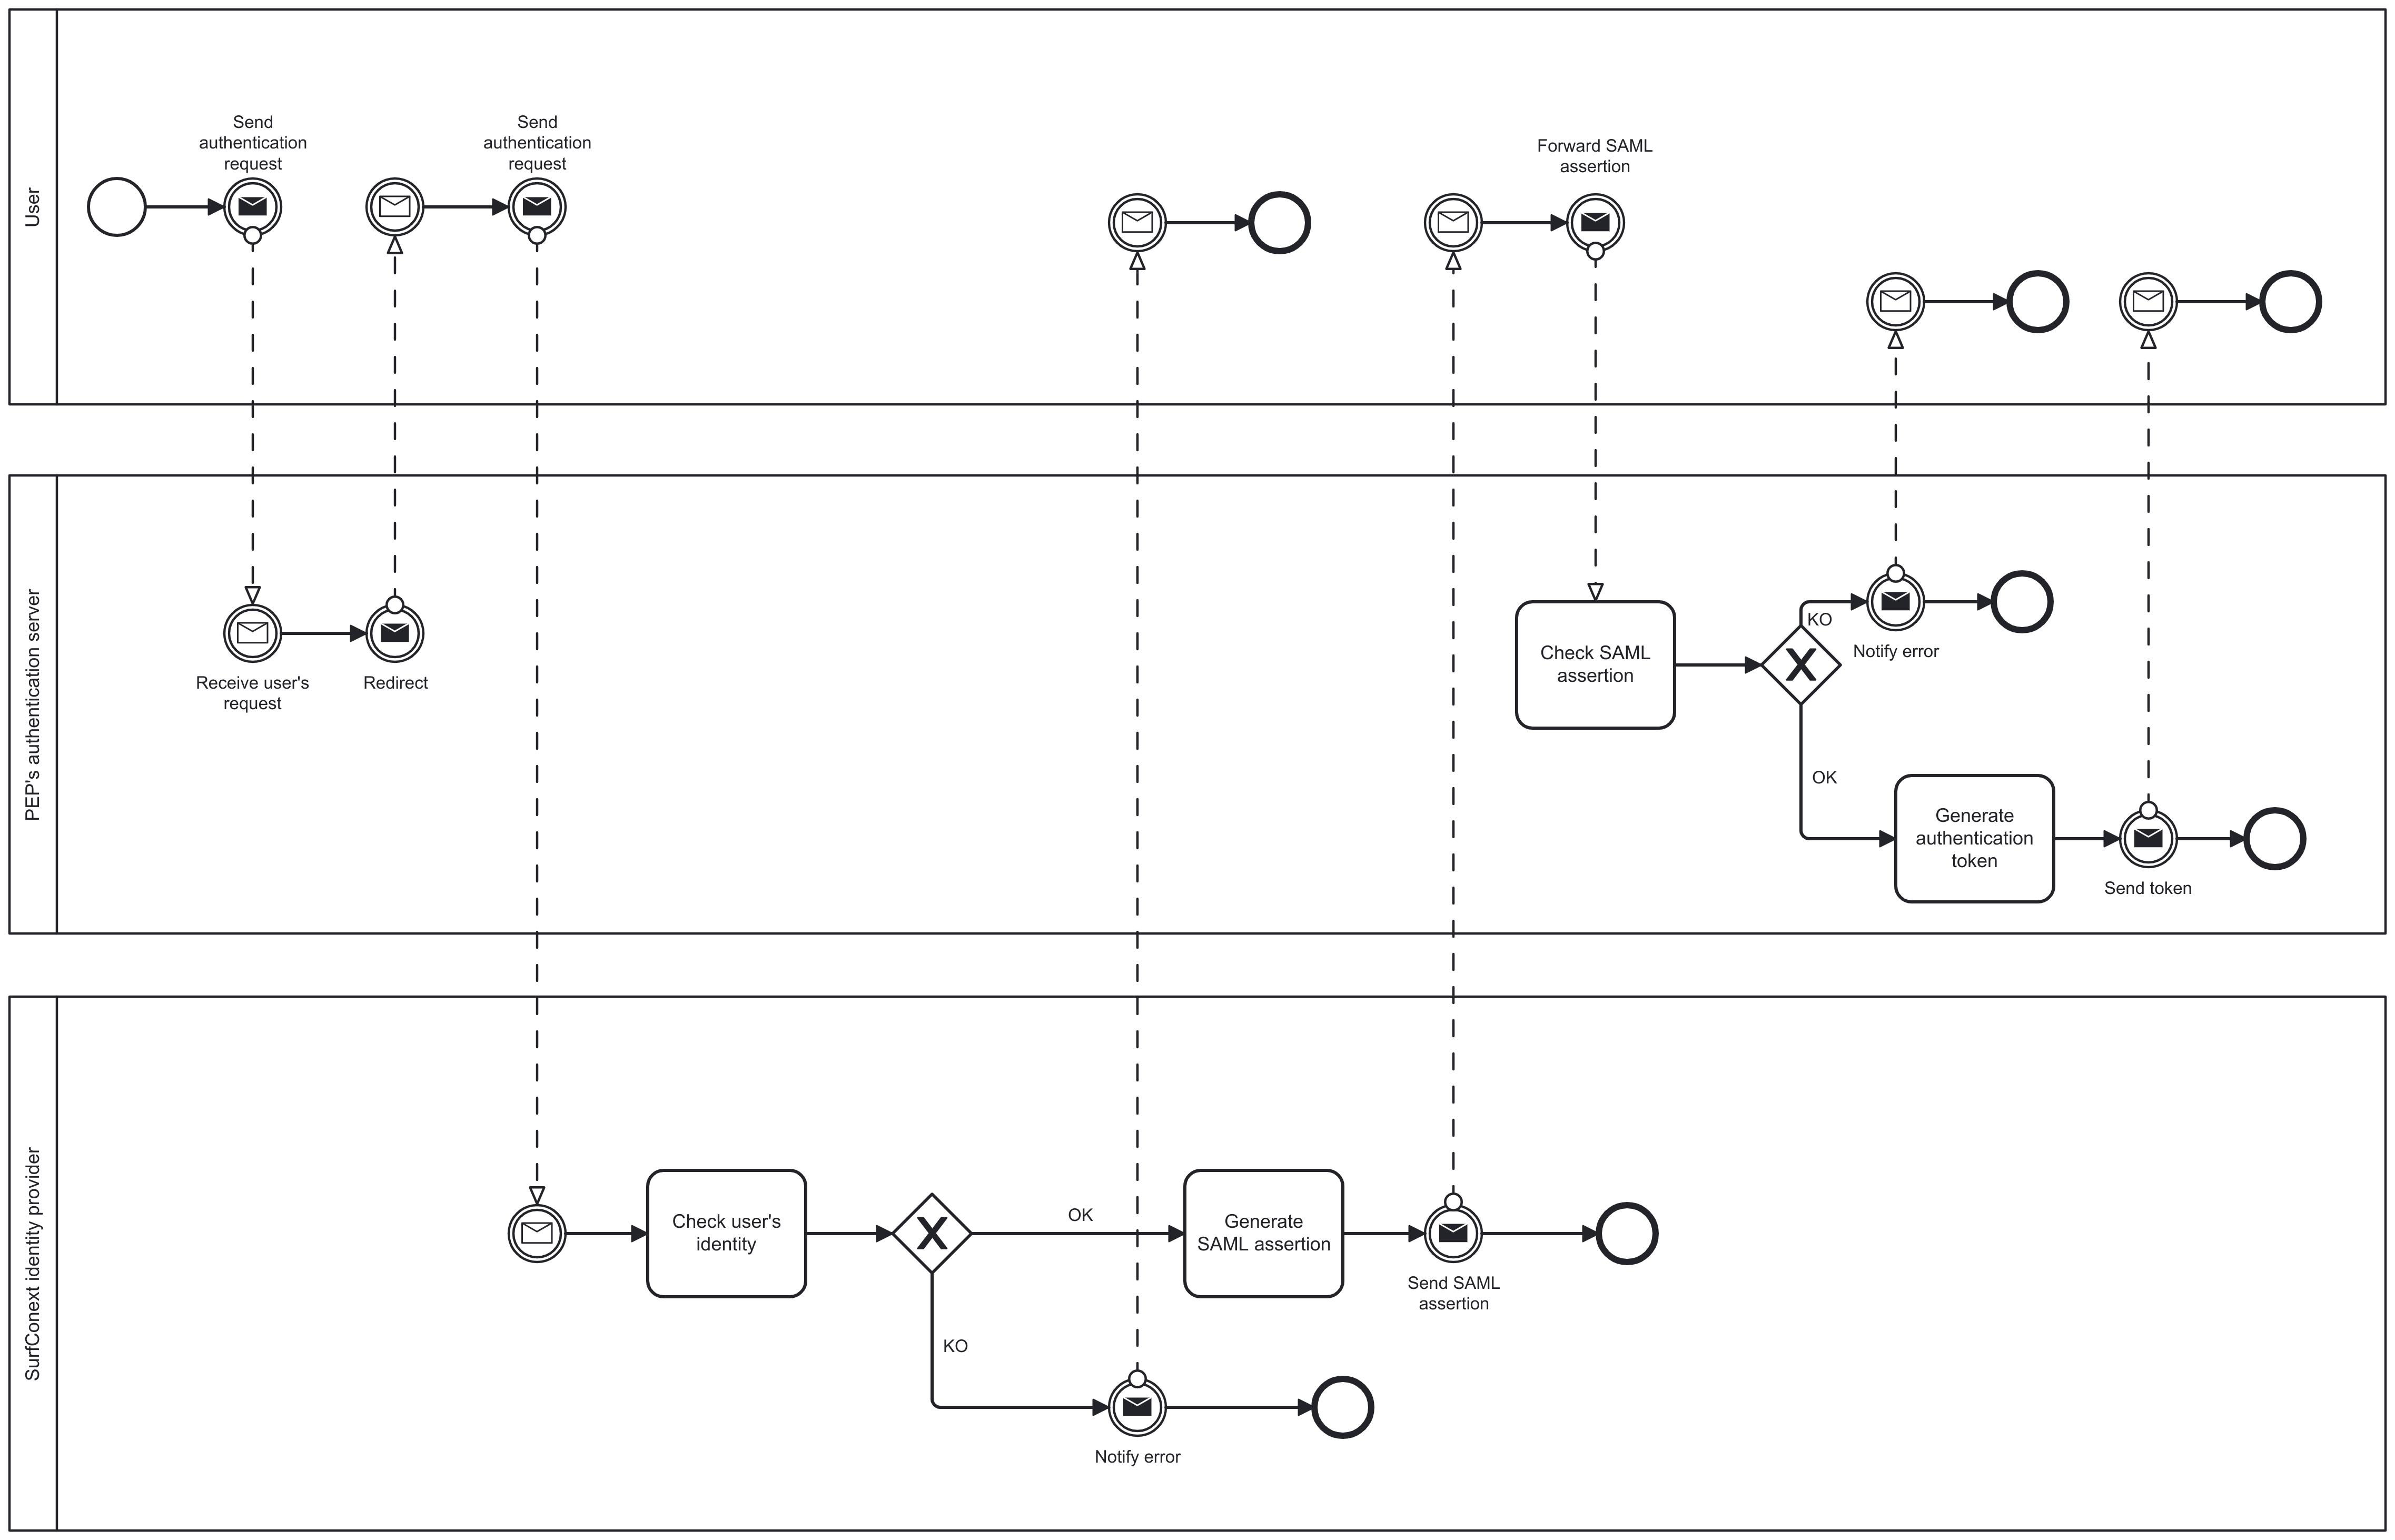
\includegraphics[scale=0.1, angle=-90]{authentication.png}
	\caption{PEP's authentication flow as a BPMN diagram}
	\label{bpmn-authentication-flow}
\end{figure}

\subsubsection{Enrollment}
In this phase, a user obtains a PEP user certificate \ref{authentication_and:authorization} and his own ElGamal private key needed to decrypt the data. \par
It starts with the user contacting PEP's key server and presenting an enrolment request. This request contains the user's authentication token and a certificate signing request.
The certificate signing request is a X509 certificate, minus the signature. If the token is valid, the certificate signing request is signed by the key server and becomes a valid
PEP user certificate. Then the user contacts the access manager and transcryptor servers, to obtain the key components. These key components are two factors that, when multiplied 
together, generate the user's private key. These factors are split between two servers (the access manager and the transcryptor, which are supposed to be managed by two different
entities), so none of the two has knowledge of the user's private key. The user multiplies the two factor, obtaining its own key.

\begin{figure}[H]
	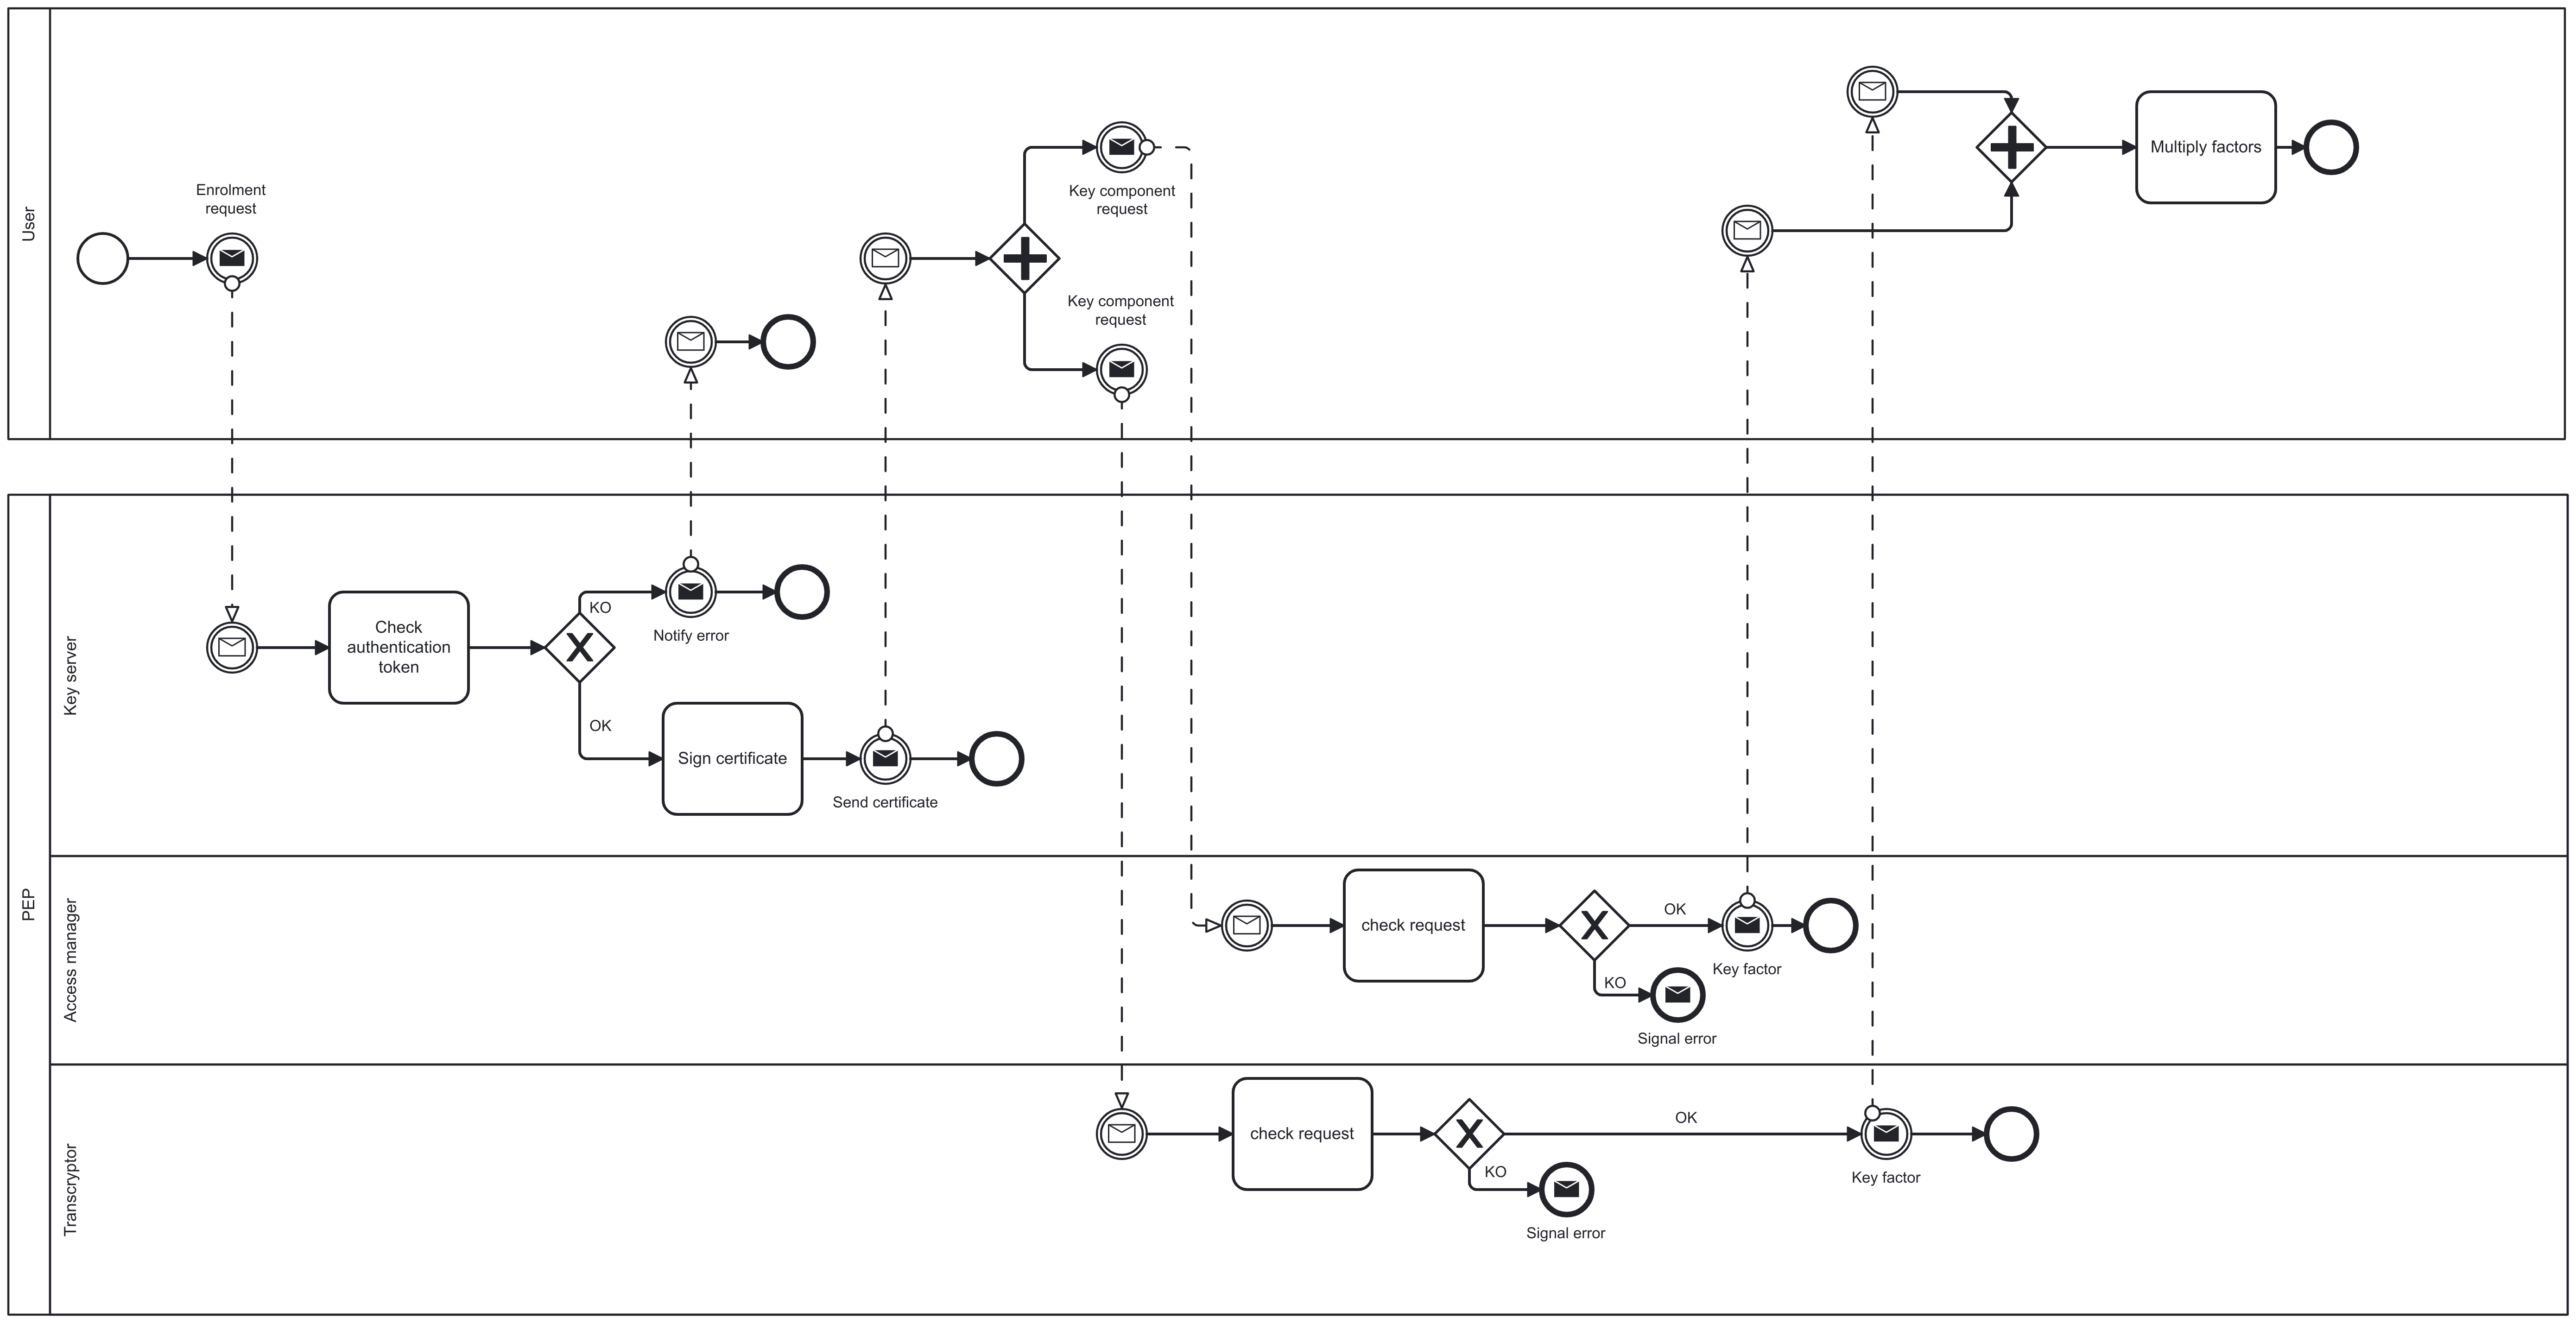
\includegraphics[scale=0.1, angle=-90]{enrollment}
	\caption{PEP's enrollment flow as a BPMN diagram}
	\label{bpmn-enrollment-flow}
\end{figure}

\subsection{pepcli}\label{pepcli}\todo{mention the commands relevant for my solution and explain what they do}
\textit{pepcli} is a command line client used to interact with PEP. It implements data access as well as all the functionalities needed for administration tasks, like adding
columns or rows to the PEP table and managing permissions. Therefore, it implements all the protocols needed to support the procedures outlined in section \ref{data_access} \enquote*{Data access}.

\chapter{Challenges and possible solutions}
\section{The issue at play}
\subsection{Authenticating study participants, but how?}
The primary goal of this work is to give study participants access to their own data, while also protecting their privacy. Secondarily, the solution should require only limited
changes to the already existing design and infrastructure of PEP, and also work for study participants that are already registered inside PEP.\par Direct access via some mechanism
external from PEP is not possible, as the data is encrypted as presented in \ref{data_structures}. This means that one has to go through PEP to get the right key and decrypt a
piece of data. So it is necessary to design a solution that integrates with the rest of PEP's architecture. Additionally, PEP's table \ref{data_structures} does not contain the
identity of participants. It instead contains pseudonyms, and the link between these pseudonyms and the participants' identities is established inside the CRM \ref{CRM}. \par 
It would be possible to write a component that sits in front of the CRM. The study participant discloses his own identity to that component using Yivi and the component uses the
disclosed identity to look up the corresponding pseudonym inside the CRM using Salesforce's API \cite{salesforce}. But, since accessing the data inside the CRM gives the ability to
deanonimyze the study participants, this access is very constrained and it would be risky to approach the CRM also as part of a solution to let participants consult their data.
Obviously, each participant must have access to its own data only, so there is the need to link a person to a specific row of PEP's table, but without (directly) using the person's
identity. \par 
A way of obtaining the needed result, could be to give study participants their own PEP ID \ref{pseudonyms} during a study's registration phase as a Yivi credential,
but this approach has been deemed to be risky by the PEP team, as it could reveal more information than needed. \par Another possibility could be to give participants a re-shuffled
\ref{elgamal_recap} version of their PEP ID, a.k.a. a local pseudonym \ref{pseudonyms}. The problem here is that PEP's table does not contain the local pseudonyms, those get
computed on-demand when someone accesses the data. So when logging in, PEP doesn't know what are the possible local pseudonyms associated to each participant\footnote{It
would need to compute all the used local pseudonyms for all the registered study participants, which is clearly inefficient.}, thus it cannot easily link a person to its row this way. \par
Another way is to add a new column to PEP's table, containing a random identifier that can be given to the study participant as a Yivi credential when they register for a study.
This would already be a working solution, as it would be possible to write a new PEP component that, during the login phase, looks at the disclosed credential and links the
participant to its own row; thus giving them access to that row only. But this would require to modify PEP's table to add an extra column. \par 
While that would be a minor change,
it can be avoided with a slightly better design: create a new user and use PEP's permission system \ref{data_access} to limit this user's access only to the row and columns containing
the medical data of the corresponding participant. The username will be the string \enquote*{participant:} prepended to a random string. The same value as the username is given as
a Yivi credential to the study participant. Then, the data administrator creates a new participant group containing only that user and the access administrator gives that user
access to that group and to the columns containing medical data. Upon login, the user discloses its Yivi credential. Since the credential's value is the same as the username
assigned to the participant, it is now possible to link the participant to its own row. Given the credential is a random identifier, it doesn't carry any information about the
person's identity. This solution features the additional advantage of not storing such random identifier inside PEP's table, which, in addition to not requiring the inclusion of a
new column into PEP's table, it also serves as a form of defence in depth protecting from researchers reading these random identifiers due to a configuration error on the access
administrator's side. In fact, if that happened, researchers would be able to trivially correlate participants across different datasets: contrary to local pseudonyms
\ref{pseudonyms}, this identifier does not change based upon the context and is instead fixed. Now we have a privacy-preserving link between a person and its row inside PEP's
table. \par
The reader may ask why prepending the string \enquote*{participant:} to a random identifier, as this solution would still work by using just the random part. The reason is that
this approach requires creating a new user, a special group containing only a specific participant and then give the new user access to this newly created group and to the columns
inside PEP's table that contain the results of medical tests. As explained in section \ref{data_access}, this would require both a data administrator and an access administrator to
be present during a participant's registration inside PEP. This can be inconvenient in practice. But, by prepending the string \enquote*{participant:} to a random identifier, a
future version of PEP
could detect that a participant is logging in, and automatically give the relative user the correct permissions without having to manually specify those for each study participant.
The exact permissions that are granted to a user to let a study participant access his own data are listed alongside the relative pepcli commands in section \todo{add ref once I
write it}.

\section{Failed attempt}
At the beginning of this work, I considered many possible solutions, that either turned out to not respect PEP's privacy standard or were deemed risky by the PEP team. Other
solutions, instead, while feasible in theory, failed in practice. This section briefly presents one of those of the latter category, as it would have made for a clean solution that
nicely integrates with the rest of PEP's architecture. Even though this attempt at a solution did not work out, some elements of it were used as part of the working solution
presented later.\par

\subsection{Design choices}
As PEP already uses the SAML standard \cite{sstc-saml-core-errata-2.0-wd-07} for authentication, it would be natural to implement a SAML identity provider using Yivi \cite{irma-app}.
Here is a BPMN diagram of the process that would be required to register a new study participant.

\begin{figure}[H]
	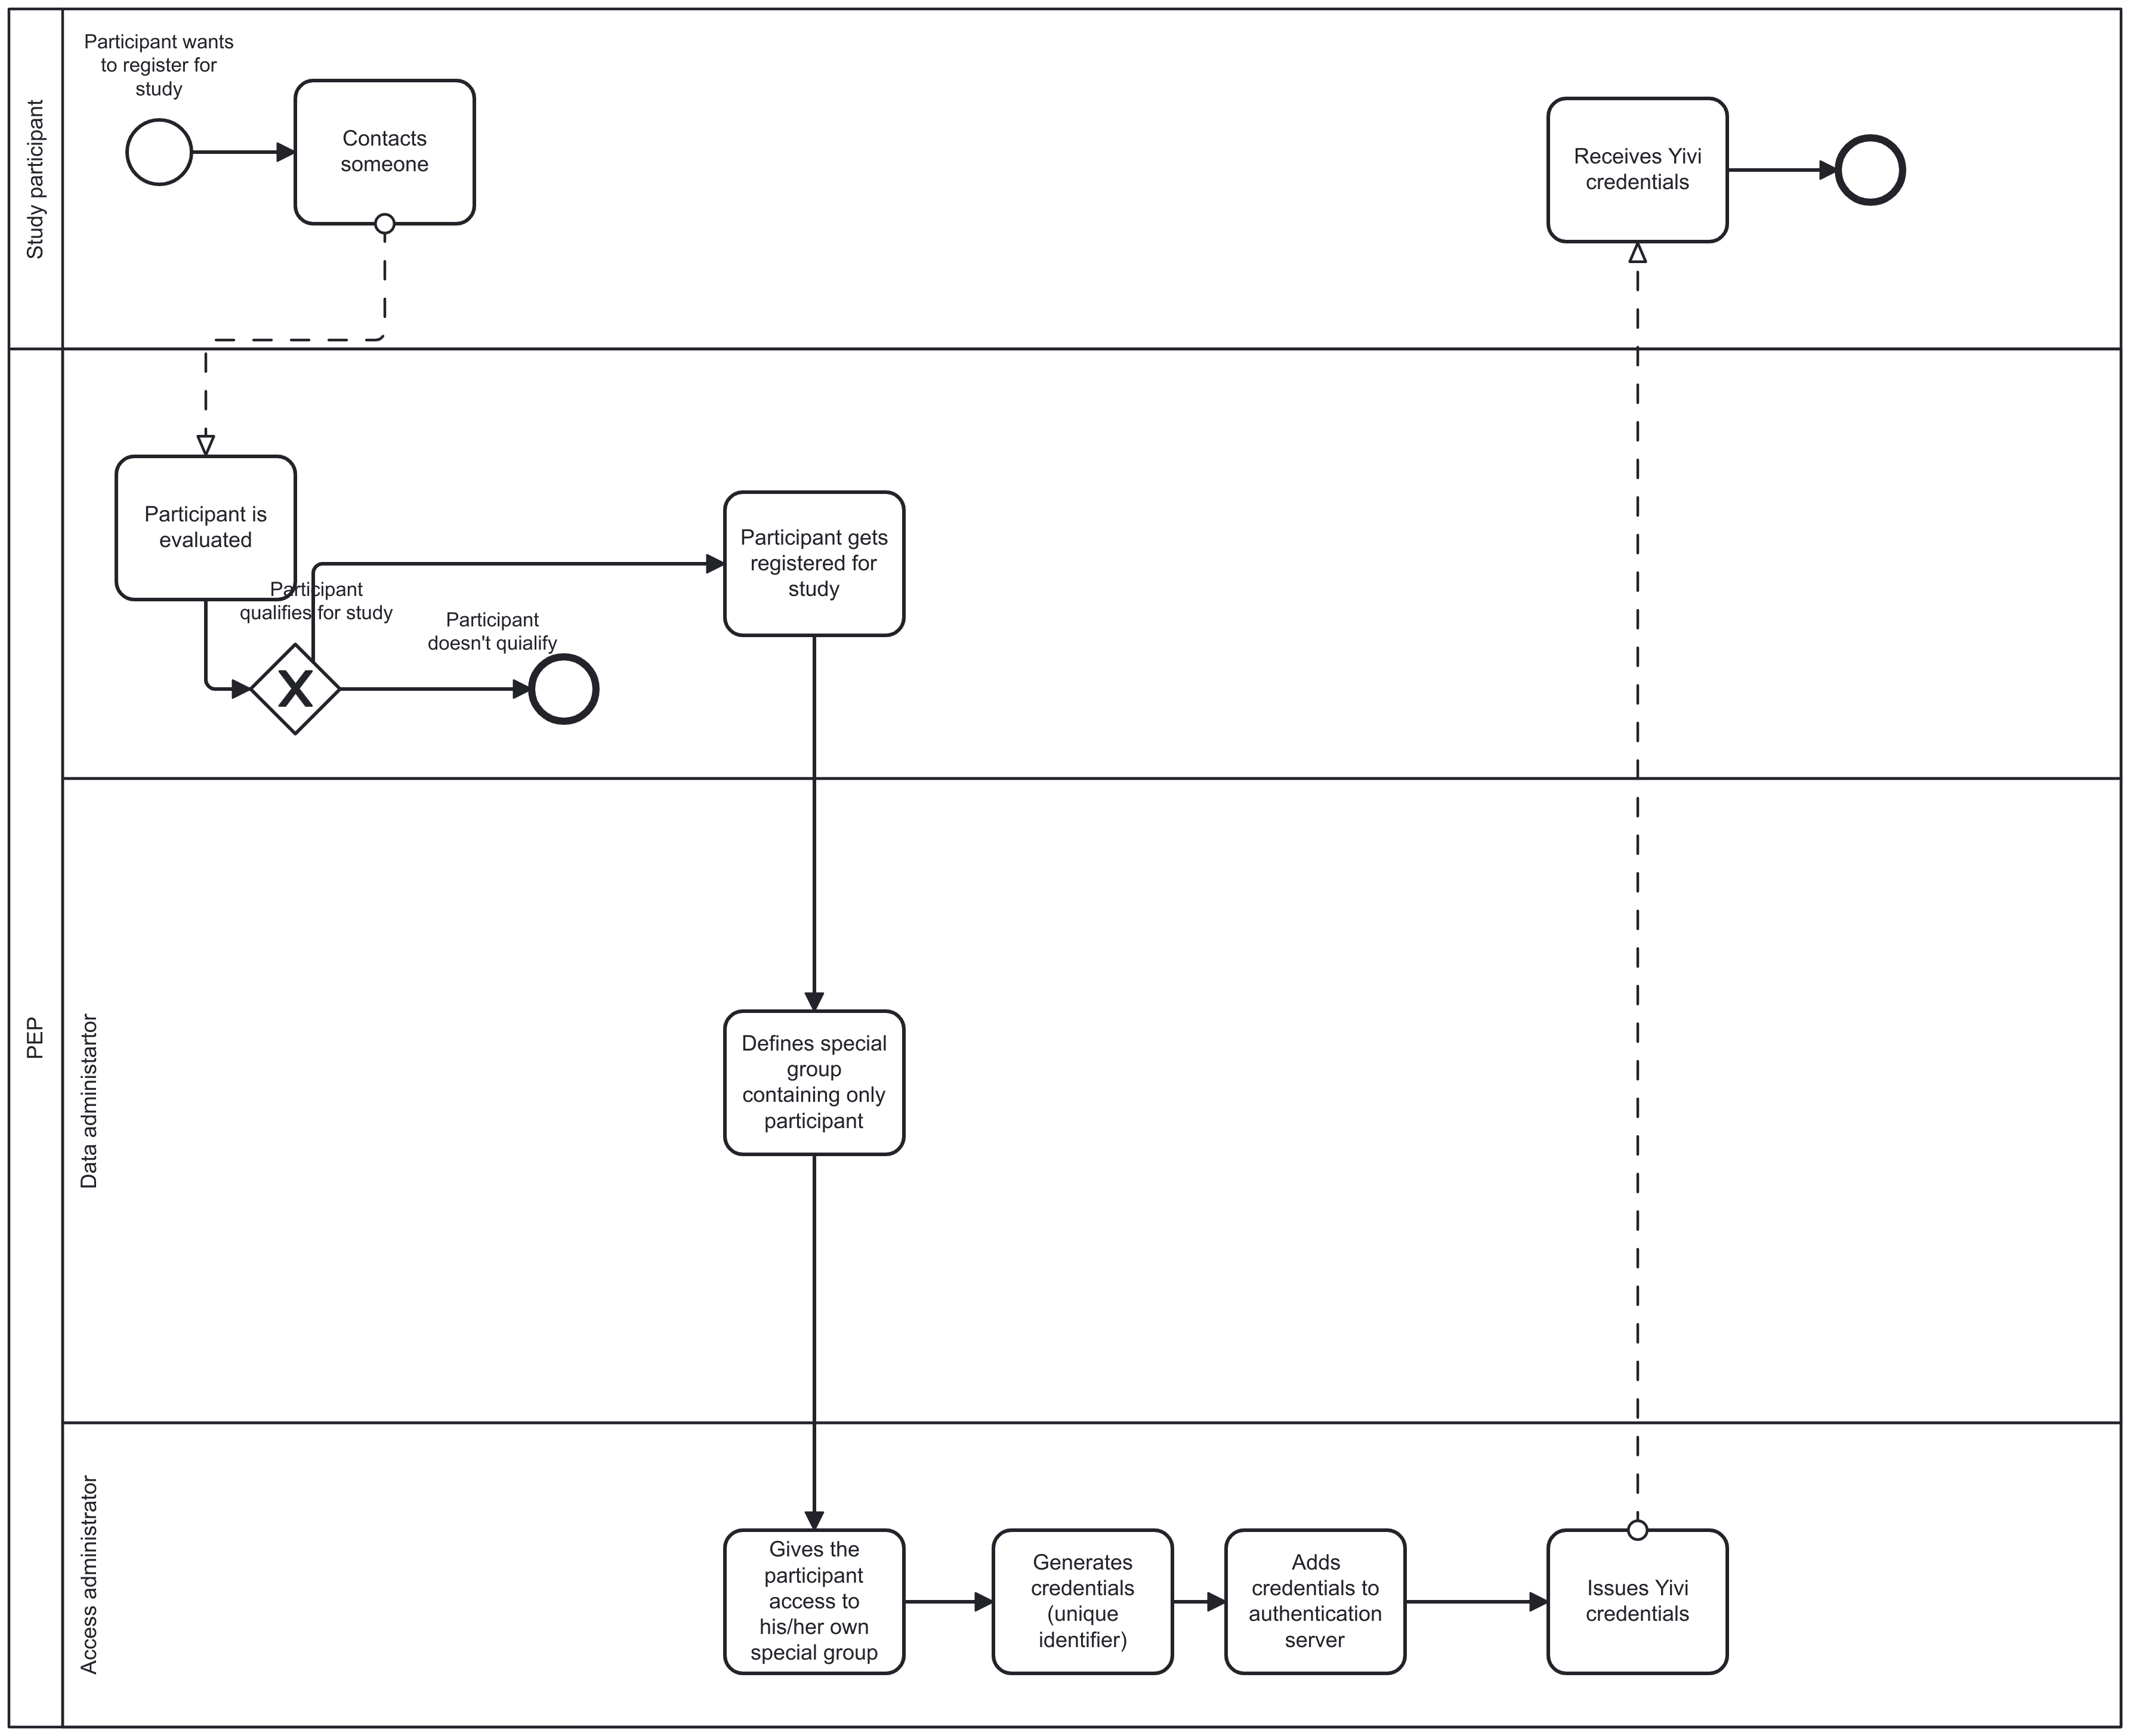
\includegraphics[scale=0.1]{registration_flow.png}
	\caption{Failed attempt registration flow as a BPMN diagram}
	\label{bpmn-registration-flow}
\end{figure}

Due to formatting constraints, the relative data access flow is available here \cite{data-access-failed-attempt-bpmn-diagram}.

This solution requires generating a credential that lets a study participant authenticate to PEP, but without leaking the participant's identity. To be in line with PEP's own
design choices, I decided to use the string \enquote*{participant:} followed by a random string as an identifier that gets linked to the participant during the registration phase. Such string is 
a version 4 UUID as described in RFC 4122 \cite{uuid_rfc}. The reason for prepending the string \enquote*{participant:} is that this makes it clear that the attribute is related to
a study participant. This can be used in the future to automatize or simplify some aspects of this login solution in the future by writing some logic specific for the case of
participants authentication. Some suggestions of where this can be applied will be presented where relevant.

\subsubsection{Version 4 UUID}\label{uuid_collision_discussion}
A version 4 UUID is a 128 bits-long value, usually represented as a string of hyphen-separated hexadecimal values. 6 bits are set to predetermined values, this leaves 122 bits of
randomness. But the goal of UUID is to have identifiers that do not collide, not to have unpredictable values. In fact, the specification says: \enquote*{Do not assume that UUIDs are 
hard to guess; they should not be used as security capabilities (identifiers whose mere possession grants access), for example. A predictable random number source will exacerbate the
situation}. So the aforementioned 122 bits of entropy have to be considered only to evaluate the robustness against collisions. UUIDs should not be considered as a secret key, as
the standard doesn't guarantee that they are hard to predict. The security against an adversary finding out a valid UUID and trying to forge a credential is given by Yivi and has
no correlation with properties of UUID other than their resistance to collisions.

\subsubsection{Estimating collision probability: the birthday paradox}
To analyze the probability of two version 4 UUIDs colliding, we apply the birthday paradox. 
This paradox answers the following question: what is the probability that two or more people share the same birthday in a group of $n$ people? It is often used in Cryptology to
establish an upper bound on the security offered by a hash function, and can be used in general to evaluate the probability of obtaining the same result twice out of a uniformly random
process. \par
To answer the paradox's question, it is easier to first compute the probability that no one has the same birthday, and then compute the complement probability. We start by ordering all 
the people in the group, and then for each of them we ask what is the probability that that person doesn't share its birthday with any of the previous ones. We will consider only years
of 365 days and assume that all days are equally likely to have births. We will further assume that each birth is an event independent of all the other births, so we are not
considering the case of twins. For the first person, the
probability is 1, since we are not considering any other person yet. Then, the probability of the second person not sharing their birthday with the previous one is the probability
that this person is born in any day of the year other than the day the first person was born in: $1-\frac{1}{365}$. For the third person, the probability of not sharing the
birthday with any of the previous two is the probability of being born in any day other than the two days already taken by the first two: $1-\frac{2}{365}$. This pattern stays
valid for any number $n$ of people\footnote{Some explanations of the problem define a special case for $n>365$. Although one can save computations by noting that if you have more
people than days in a year then you must have a collision, the general formula still works since one of the factors becomes zero.}, so the probability that in a group of $n$ people no-one shares its birthday with another person of the same group is $1(1 - \frac{1}{365} ) \dotso  (1 - \frac{n - 1}{365} ) = \prod_{k=1}^{n-1}(1-\frac{k}{365})$. From this follows that 
the probability of having at least two people that share their birthday in a group of $n$ people is

$$P("Same\ birthday")=1-\prod_{k=1}^{n-1}(1-\frac{k}{365})$$

The birthday paradox is called as such because, using the previous formula, we can see that when considering a group of 23 people we already get a $50\%$ chance of two of
them sharing their birthday. This outcome is counter-intuitive, because 23 looks much smaller than $365/2=182.5$. \par

This result can be generalized to obtain a formula we can use for the case of version 4 UUID collisions. Instead of considering birthdays, let's consider the case of a group of $n$
people randomly choosing an object from a set of $u$ objects, with replacement. Here $u$ is the set of all possible version 4 UUIDs. Following the same reasoning as before, we obtain
$1(1-\frac{1}{u}) \dotso (1-\frac{n-1}{u}) = \prod_{k=1}^{n-1}(1-\frac{k}{u})$. So the probability of having at least two version 4 UUIDs colliding is

\begin{equation}\label{uuid_collision_exact_formula}
P("Collision")=1- \prod_{k=1}^{n-1}(1-\frac{k}{u})
\end{equation}

Computing the exact value for large values of $n$ and $u$ is prohibitive. For this reason, it is often used an approximation of the above formula. To derive it, we have to look at the
problem from a slightly different perspective. Let's imagine to have a box containing all the possible UUIDs. For each person, we pick a UUID from the box, write it down to assign
it to that person and then put it back in the box. We also re-shuffle the content of the box before extracting a new one, otherwise recently-extracted UUIDs would have a higher
chance to be extracted compared to new ones. To see if there are collisions, we now consider all the possible pairs of people, and ask 
for each pair if the two UUIDs are the same or not. Each comparison is a Bernoulli trial, so when we consider a sequence of such comparisons we obtain a binomial distribution.
Let's introduce a random variable $X$ counting the number of collisions. We have that $X \sim B(m,p)$, where $m$ is the cardinality of the set of all possible pairs and $p$ is the
probability that a given pair represents a collision. So $m=\binom{n}{2}$ and $p=\frac{1}{u}$. We can now use the binomial distribution's probability mass function to compute the
probability of finding $k$ collisions: 
$$P(X=k)=\binom{m}{k}p^k(1-p)^{m-k}$$
By substituting the expressions for $m$ and $p$, we get
$$P(X=k)=\binom{\binom{n}{2}}{k}(\frac{1}{u})^k(1-\frac{1}{u})^{\binom{n}{2}-k}$$
We can now see that the probability of having no collisions is
$$P(X=0)=(1-\frac{1}{u})^{\binom{n}{2}}$$
And so the probability of finding at least a collision is:

\begin{equation} \label{uuid_collision_binomial_approximation}
		P(X \geq 1)=1-P(X=0)=1-(1-\frac{1}{u})^{\binom{n}{2}}
\end{equation}

We can notice an issue with this modeling of the problem: formula \ref{uuid_collision_exact_formula} was correctly telling us that, if we generate more UUIDs than the number of
possible distinct UUIDs, we must get a collision. In this new formulation of the problem instead, the term $(1-\frac{1}{u})^{\binom{n}{2}}$ will approach zero for increasing values of
$n$, but will never be \emph{exactly} zero. So formula \ref{uuid_collision_binomial_approximation} will never give us absolute certainty of finding a collision. This behavior
results from modelling each attempt at finding a collision as a Bernoulli trial. For an experiment to be a Bernoulli trial, it must satisfy two conditions: 
\begin{enumerate}
		\item The experiment admits only two, mutually-exclusive, outcomes
		\item Repeating the experiment multiple times does not change the probability of the outcomes
\end{enumerate}
Here the issue arises due to the second condition: it holds if we are generating an amount of UUIDs which is less or equal to the total number of possible UUIDs, but it trivially
breaks down if we generate more UUIDs than the number of possible distinct UUIDs. We can fix it by considering these two cases separately:

\begin{equation} \label{uuid_collision_binomial_model}
		P(X \geq 1)=
		\begin{cases}
				1-(1-\frac{1}{u})^{\binom{n}{2}} & n \leq u \\
				1 & n > u
		\end{cases}
\end{equation}

This is still not the expression we are looking for, as again computing its outcome for big values of $u$ and $n$ is computationally intensive.
But, while rewriting the result in this form does not help computing it per se, we can now use the fact that this is a binomial distribution to apply a Poisson approximation. If we have
a binomial distribution of parameters $n$ and $p$ where 
\begin{equation}\label{condition_for_poisson_approximation}
	n \geq 20 \land p \leq 0.05 \lor n \geq 100 \land p \leq 0.1 
\end{equation}
a Poisson distribution of parameter $\lambda=np$ is a good approximation \cite{source_for_poisson_approximation}. Under this assumption, we can say that the
probability of not having collisions is

\begin{equation}
		P(X=0)=
		\begin{cases}
			e^{-\lambda} & n \leq u \\
			0 & n > u
	\end{cases}
\end{equation}

and, finally, the probability of having at least one collision is

\begin{equation} \label{uuid_collision_poisson_approximation}
		P(X \geq 1)=
		\begin{cases}
				1-e^{-\lambda} & n \leq u \\
				1 & n > u
		\end{cases}
\end{equation}

where $\lambda=np$.\newline

We can empirically see how close these different modelings of the problem are to each other by plotting the results for the case of $365$ possible birthdays or objects.

\begin{figure}[H]
		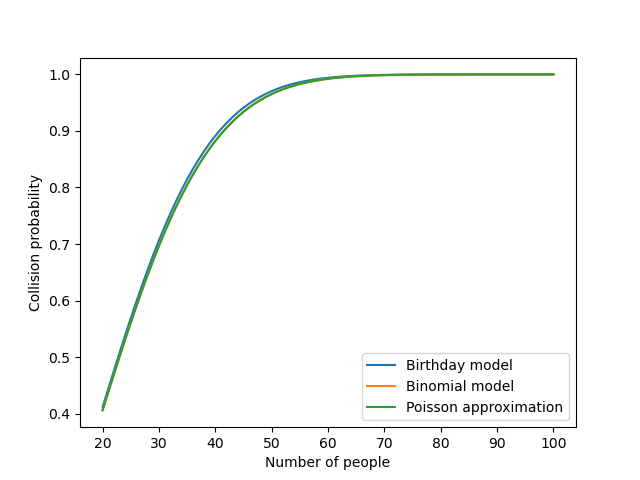
\includegraphics[scale=0.5]{Exact probability vs approximations}
		\caption{Probability of finding at least one collision when picking from a set of 365 object, computed with the methods presented above for groups from 20 to 100 people}
\end{figure}
\noindent
The above graph shows that the binomial model is equivalent to the one obtained by applying the birthday paradox. Furthermore, when condition \ref{condition_for_poisson_approximation} is satisfied, the
Poisson approximation allows us to get a result close to the exact value while being much less expensive to compute.

\subsubsection{Application to version 4 UUID}
Version 4 UUIDs are 128 bits long, of which 6 are fixed and 122 are randomly generated. So we have $u=2^{122}$ possible UUIDs. Assuming a uniformly random number generator is used, this gives us
$p=\frac{1}{u}=\frac{1}{2^{122}}$. So the condition on $p$'s value is satisfied. We can easily see from any of the previous modelings of the problem that, the more UUIDs get generated, the more likely it is to find a
collision. This nice fact lets us consider worst-case scenarios while also satisfying the condition on the value of $n$ that makes the Poisson approximation close to the exact result,
saving us quite a lot of computations. Let's then consider two extreme cases and see what the probability would be to have a collision. \par
The first case is to generate one UUID for each person in the world. At the time of writing, the global population is estimated to be around \num{8088000000} people
\cite{world-population}. By plugging these numbers in formula \ref{uuid_collision_poisson_approximation}, we obtain that in this scenario

	$$P("Collision")=1-e^{-\lambda}=1-e^{-\frac{8088000000}{2^{122}}} \approx 1.52 \times 10^{-27}$$

The second scenario is to have each person in the world taking part in 100 studies and getting a separate credential for each one of them (or, equivalently, the world population
increasing 100 times). By using formula
\ref{uuid_collision_poisson_approximation} again, we get

$$P("Collision")=1-e^{-\lambda}=1-e^{-\frac{808800000000}{2^{122}}} \approx 1.52 \times 10^{-25}$$ 

Both results are negligible. For comparison, the probability of dying in a given year due to an asteroid impact is estimated to be between $3.33 \times 10^{-8}$ and $5 \times
10^{-7}$, depending on the type of impact \cite{death-by-asteroid}.

\subsubsection{Yivi} \label{yivi}
Yivi is a project maintained by the Privacy by Design Foundation \cite{privacybydesignfoundation} implementing the Idemix anonymous credential system \cite{idemix_specification}. It
lets an \textit{issuer} issue a credential that can subsequently be verified by a \textit{verifier}. The idea behind this system is that a service may need to know some
information about a person before offering this person a service, without the need to know other information, related but not relevant, that is usually provided with traditional
identification methods. E.g. a shop needs to verify that a person is over 18 years old before selling an alcoholic beverage to that person, but it doesn't need to know the exact age of
that person, his name and all the other information that is typically present on traditional identity documents. Yivi provides a way to disclose only a specific piece of
information (in this case that a person is over 18), called an \textit{attribute}, without leaking any additional information \cite{irma-docs}. \par
Summarized, it works by having a trusted third party act as an issuer. This party is in charge of verifying that a person has a certain characteristic (i.e. being over 18 or being
a student) and then issuing the relative Yivi attribute to that person. Later, a verifier can contact an Yivi server to have it generate a disclosure request. The user reads this
request using his Yivi app and, if he agrees to disclose the requested attribute, the Yivi server validates the corresponding credential and lets the verifier know the value of the
requested attribute. More details can be found in Yivi's documentation \cite{irma-docs}. \par
Using Yivi has the advantages of offloading the actual authentication to a solid and privacy-preserving project, while providing at the same time a simple user experience: when
authenticating via Yivi, a user has just to scan a QR-code with the Yivi app and confirm his will to disclose the requested attribute. \par
The Yivi server periodically retrieves a list of valid attribute types from a centralized repository. Similarly, the Yivi app does not accept to store attributes not present in such
centralized repository. To have one's credential added to this repository, one needs to create a pull request on a GitHub repository and pay the Privacy by Design Foundation a
yearly fee \cite{irma-docs-issuer}. An alternative is to use demo credentials. It is possible to host an Yivi server with a locally-modified copy of the demo credentials
repository. These are credentials that only work for testing purposes and do not work on production systems. As an additional safety measure, the Yivi app does not work with such
credentials unless developer mode is activated and one compiles his own version of the app with such credentials added to the local demo repository used while compiling the app. \par 
To implement my proof of concept, I set up a local Yivi server with a demo credential called \enquote*{irma-demo.PEP.id} and I compiled my own version of the Yivi app with
this credential baked-in. This works for showing that my solution works, but if in the future the PEP team decides to use this or a similar one in production, there is the need to
contact the Privacy by Design Foundation to register a production credential.

\subsubsection{The Rust programming language and memory safety} \label{rust_memory_safety}
This solution requires writing some custom code, so we needed to choose a suitable programming language. In such a choice, there's always a subjective element and, for me, it was
the curiosity of learning this recent language. Subjective judgment aside, there are also good objective reasons to pick Rust. \par
PEP's codebase is written in C++, so we either need to use C++ itself or a language that nicely integrates with a C++ codebase. Additionally, PEP focuses on security, since it
handles medical data. Rust aims at being a substitute for C and C++ while also offering strong safety guarantees, with a special focus on memory safety. It is also designed to fit
with pre-existing C and C++ code. \par
Memory safety is a property of some programming languages that perform memory management in such a way to prevent errors like segmentation fault and double free. A computer's
available volatile memory is split into two parts: a stack and a heap. While most programming languages take care of automatically managing the data that lives on the stack,
managing the heap memory is more complicated: when using the stack, data is always added on the top and removed from the top of the stack (first in first out policy); when using the heap instead, the data can
be stored anywhere there is enough free space, and when the memory is not needed anymore it needs to be returned to the allocator. Although storing data on the heap always needs to
be done explicitly (either by directly invoking an allocator or by calling a class' constructor), freeing no-longer-needed memory can be approached in two different ways: either provide an automatic mechanism to free such memory, usually in the form of a
garbage collector, or leave to the programmer the responsibility to free unused memory at the right time. The former approach is memory-safe, but it comes at a performance cost,
while the latter can be very efficient but it is also error-prone. \par
There are two types of memory safety: spatial and temporal \cite{eternal-war-in-memory}. Spatial memory safety prevents attempts at accessing the wrong regions in memory. For example, segmentation faults and
buffer overflows are violations of spatial memory safety: the former because it is the result of an attempt of accessing an invalid memory address, the latter because it is an
attempt at writing to a memory region more data than what it can contain, resulting in a write past its boundary. Temporal memory safety ensures that a program
can only access valid data, and when a piece of data becomes invalid it is not accessible anymore. Examples of violations of temporal memory safety are double-free errors and
dangling pointers. A double-free error is when \enquote*{free()} is called twice on the same memory region. This corrupts the program's memory management structure and can cause
the program to crash or to alter its execution flow \cite{double-free}. A dangling pointer is a pointer to a memory region that has been freed. Using such memory leads to undefined
system behavior. \par

Rust aims at ensuring both temporal and spatial memory safety, without a meaningful performance hit. The core mechanism that allows Rust to accomplish this is the concept of
ownership. Ownership is a set of rules defining how Rust manages memory. These rules ensure memory safety and are checked by the compiler at compile-time, so they carry no
performance cost while the program is running. The fundamental observation at the core of those rules is that there's a natural place where memory can be deallocated, and it is when
a value goes out of scope, thus it cannot be accessed anymore. Here are the main ownership rules, taken from \cite{rust_ownership_rules}:

		\begin{itemize}
				\item Each value in Rust has an owner.
				\item There can only be one owner at a time.
				\item When the owner goes out of scope, the value will be dropped.
		\end{itemize}

These rules are enforced by the borrow checker. It is a static analyzer inside the Rust compiler that makes sure no reference outlives the data it is pointing to. It also ensures
that only one reference at a time is able to modify the underlining data. In Rust, a reference is a fat pointer \cite{eternal-war-in-memory}, i.e. a pointer that, along with a memory address it
is pointing to, it also carries additional information like the maximum amount of data that can be stored at that memory location and how much data is already stored there. This
makes it possible to perform runtime checks to guarantee that read and write operations only happen within the bounds of the memory region referred by the pointer. 
Every time a value is bound to a variable, that variable takes ownership of the underlying data, and when the owner, i.e. the variable, gets out of scope the relative memory is
freed. Let's consider a simple example:

\begin{lstlisting}[language=Rust, style=colouredRust]
	{
		let x=42;
		let string=String::from("Lorem ipsum");
	}
\end{lstlisting}

The curly braces define a new scope. In this scope, two variables are defined: one holding an integer value and another holding a reference to a string. In both cases, when the
program execution reaches the closing curly brace the memory where the data is stored gets freed. \par
Rust's behavior gets a bit more involved when assigning the value of a variable to another variable. Consider the following example:

\begin{lstlisting}[language=Rust, style=colouredRust]
	{
		let x=42;
		let y=x;
		let string1=String::from("Lorem ipsum");
		let string2=string1;
	}
\end{lstlisting}

Here we observe two different behaviors, depending on whether a value is stored on the stack or on the heap. The variable \enquote*{x} is an integer, thus it is stored on the
stack. Similarly to other programming languages, since this value lives on the stack, the statement \enquote*{let y=x} copies the value of \enquote*{x} into \enquote*{y}. Since we
now have two independent copies of the value \enquote*{42}, there is no issue in deallocating the used memory at the end of the scope. The variable \enquote*{string1} contains instead
a pointer to a string stored on the heap. Since duplicating heap data can be expensive, the statement \enquote*{let string2=string1} copies the pointer data from
\enquote*{string1} into \enquote*{string2}, without allocating a new string. But this could be a problem, as now we have two pointers to the same memory region, and trying to deallocate both at the end of the
scope would result in a double-free bug. To prevent this issue, the statement \enquote*{let string2=string1} doesn't just copy the pointer data, but it also invalidates the
variable \enquote*{string1}. Since \enquote*{string1} is no longer valid, when the program reaches the end of the scope only \enquote*{string2} is deallocated, and there is no
double-free. What happened from an ownership perspective, is that \enquote*{string1} was the original owner of the string, then the string got \enquote*{moved}\footnote{Rust uses
the verb \enquote*{to move} to indicate an assignment that results in an ownership change of the involved value} inside \enquote*{string2} which
became the new owner. If we need two separate copies of the same heap data, we have to explicitly ask for it by invoking \enquote*{clone()}:

\begin{lstlisting}[language=Rust, style=colouredRust]
	let string1=String::from("Lorem ipsum");
	let string2=string1.clone();
\end{lstlisting}

In this case, we have two distinct copies of the string. \par
Passing values to a function works analogously to assigning a variable's value to another variable: stack data is copied, while heap data is passed by reference. This means that, in
the case of heap data, the function becomes the new owner\footnote{It also owns the stack data, but since this data gets duplicated in this case the original owner does not lose
ownership of its copy.}. Consider the following example:

\begin{lstlisting}[language=Rust, style=colouredRust]
	fn main(){
		let x=42;
		let string=String::from("Lorem ipsum");
		function(x, string);
		let y=x;
		let string2=string;
	}
	fn function(mut answer: i32, mut latin: String){
		answer+=1;
		latin.push_str(" dolor sit amet");
	}
	
\end{lstlisting}

This example does not compile, as it violates ownership's rules. The variable \enquote*{x} behaves like in most programming languages: the function makes its own copy of the value
42, increases it and when the function returns it gets deallocated. So when \enquote*{y} is assigned the value of \enquote*{x} after the function call, it gets the original value
of 42. The problem lies with the string. In Rust's terminology, the string is \textit{moved} inside the function, i.e. the function takes ownership of the string without making a
copy of the underlying data. This means that the string gets deallocated when the function returns, and it is no longer valid after the function call. Trying to compile this code
fails with an \enquote*{use of moved value} error.\par

One way of recovering values from inside a function is to return them. In this case, a function takes ownership of the values and then gives ownership back. Here is how it would
look like:

\begin{lstlisting}[language=Rust, style=colouredRust]
    fn main(){
    	let x=42;
        let string=String::from("Lorem ipsum");
        let (y, string2)=function(x, string);
    }

    fn function(mut answer: i32, mut latin: String) -> (i32, String){
        answer+=1;
        latin.push_str(" dolor sit amet");
        (answer, latin)
    }          
\end{lstlisting}

This example compiles successfully, as returning a value transfers its ownership to whatever variable it gets assigned to. In this specific example, we are using a tuple to return
two values at once. Note also the use of the \enquote*{mut} keyword: by default, Rust variables are immutable, if something needs to be modified we need to explicitly declare a
variable as mutable using \enquote*{mut}. \par

Taking ownership of a value and then returning it every time that a function has to do some elaboration can be cumbersome: suppose we need to implement a function that says whether
a string is palindrome or not. We would need to take ownership of the string and then return a tuple with both the original string and a boolean representing the answer, despite
the fact that what we need from the function is just the boolean. This is where references and borrowing come into place. In Rust, a reference is a pointer that is guaranteed to be
valid for its whole lifetime. Using a reference, we can \textit{borrow} a value: we can access it but without taking ownership of the value. Just like variables, also references
are immutable by default, if we need to be able to change a value we need to explicitly ask for a mutable reference using the \enquote*{mut} keyword. Here is the previous example,
rewritten using mutable references:

\begin{lstlisting}[language=Rust, style=colouredRust]
    fn main(){
       	let mut x=42;
        let mut string=String::from("Lorem ipsum");
        function(&mut x, &mut string);
        let y=x;
        let string2=string;
    }

    fn function(answer: &mut i32, latin: &mut String){
       	*answer+=1;
        latin.push_str(" dolor sit amet");
    }	
\end{lstlisting}

Note that, since we are using references to mutate variables, we need both to ask for mutable references and declare the variables as mutable. Otherwise, the Rust compiler refuses
to compile the code. To retain memory safety when using references, Rust's borrow checker analyzes the code to ensure the following two conditions are valid
\cite{rust_ownership_rules}:

\begin{enumerate}
		\item At any time and for a given variable, there can be either exactly one mutable reference (and no immutable ones) or any number of immutable references.
		\item References must be valid for their whole lifetime.
\end{enumerate}

The rationale for the first condition is preventing data races, while the second condition prevents dangling pointers. \par
Using a memory-safe programming language does not guarantee to have bug-free code: this can only be guaranteed by formal verification. For example, a memory-safe language does not
help with logic bugs, i.e. errors caused by a developer coding the wrong procedure to obtain a given result. But it eliminates many common programming
mistakes that often lead to security vulnerabilities: according to the Microsoft Security Response Center, about 70\% of the security vulnerabilities in the Microsoft software
ecosystem that got assigned a CVE ID \cite{cve_id} between 2006 and 2018 were due to memory corruption bugs \cite{proactive_approach_to_safety}. This shows how memory-safe programming 
languages carry a great potential in helping develop secure software, and are therefore a natural choice when one of the main focus point of a software project is security. By
using a memory-safe language, developers can significantly reduce the number of security vulnerabilities in their code and improve the overall security posture of their software. 


\subsection{Implementation}\label{failed_implementation}
\subsubsection{Registration component}\label{registration-component}
To implement this, there is the need to write a registration component that integrates with the current PEP participants registration flow. This component is in charge of
generating credentials for study participants and issuing the corresponding Yivi cards. PEP already uses a web application as part of the registration procedure, so we opted for
writing a web application in Rust. This application has three main components: a front-end in charge of rendering a simple interface and a back-end which is further divided into
two components: one in charge of generating the attribute values and another handling the requests to the Yivi server. To build the front-end I used the Rocket web framework
\cite{rocket}; while to generate UUIDs I used the uuid \cite{uuid_crate} library crate\footnote{In Rust's terminology, a crate indicates a project and can be of two different kinds:
a library crate is a project that compiles to a library, while a binary crate is a project that compiles to an executable.}. Aiming to minimize the dependencies, the code uses the
operating system's random number generator to generate version 4 UUIDs. To handle communication with the Yivi server I used the irma\footnote{IRMA was the former name of the Yivi
project. At the time of writing, this library has not been renamed to Yivi yet.} library crate \cite{irma_crate}, and to generate the QR-code containing the Yivi card generated by
the Yivi server I used the qrcode library crate \cite{qrcode_crate}. For an exhaustive list of all the dependencies, see \cite{registration_poc_cargo_toml}. The credential
generation flow is as follows. When the application starts, it exposes an HTTP endpoint and waits for connections. Upon receiving a connection, it generates a string made by
prepending the string \enquote*{participant:} to a version 4 UUID. Then it contacts a local Yivi server listening on port 8088, and asks it to generate a new Yivi card for the
attribute \enquote*{irma-demo.PEP.id} with the generated string as the attribute's value. If the Yivi server answers with the requested attribute, the application generates a
QR-code that the study participant scans to import the newly generated credential in their Yivi wallet.\footnote{Yivi calls \enquote*{wallet} its credential store} It also shows the attribute's value, so that PEP can
be configured to link the credential to the right user\footnote{The configuration details are not provided in this section, as this attempt failed. But it would have been analogous
to the configuration presented in}\todo{add ref inside footnote once I write (and explain) the config}. Here is a BPMN diagram showing the flow:

\begin{figure}[H]
		\includegraphics[scale=0.1]{credential issuing.png}
		\caption{Flow to issue a new Yivi credential for a study participant. The piece implemented as part of this work is highlighted in orange.}
\end{figure}

\subsubsection{Security evaluation}
Since this component is executed as part of the participants registration procedures by PEP administrators, it is run in a trusted environment. The participant is present during
the registration procedure, so there is no concrete risk of assigning the generated credential to the wrong person. Here the main security risk is represented by the uuid library crate
\cite{uuid_crate}: we need that the generated UUIDs do not collide. If there is a bug in this library that results in generating the same UUID more than once, it would cause having
multiple participants with the same credential, so they would get access to the same data. In other words, if two participants get the same credential, one of them would get access
to the data of the other instead of his own. So the security of this component relies on this library being a correct implementation of the UUID version 4 standard \cite{uuid_rfc}.
Assuming the library is a compliant implementation of the standard, the discussion in section \ref{uuid_collision_discussion} shows that we can expect that we will not get colliding UUIDs.

\subsubsection{SAML identity provider}
To let a study participant log-in with the Yivi credential in his possession via SAML, we need a SAML identity provider supporting Yivi. To implement this, I tried setting up
SimpleSAMLphp \cite{simplesamlphp} to work as an Yivi \cite{about-irma} identity provider. SimpleSAMLphp can work both as a service provider and as an identity provider, and can be
extended by writing PHP plugins. There were already two previous attempts about writing such a plugin: \enquote*{simplesamlphp-module-authirma} \cite{simplesamlphp-module-authirma}
by the Privacy by Design Foundation \cite{privacybydesignfoundation} and \enquote*{irma-idp} \cite{irma-idp} by SURF \cite{surf}.  Both appear to be unmaintained, but I first
attempted to use those as a basis for my own implementation. \par I started by setting up a local Yivi server inside a Docker container and creating a demo credential
\cite{irma-docs-issuer} for PEP study participants, called \enquote{irma-demo.PEP.id}. I then tried making \enquote*{simplesamlphp-module-authirma} work again. It was developed at
a time when the Yivi HTTP server and the Yivi JSON API server where two separate components. While trying to make it work again, I stumbled upon the problem of getting the keys for
the API and web servers. Probably the key is the same for both, as now the irmago server \cite{irma-docs-server} implements both, but I was not able to find the certificate in the
required format inside my Docker container. \par After failing to make \enquote*{simplesamlphp-module-authirma} work again, I did some more research on previous work and found out
about \enquote{irma-idp}. It is more recent and, while it still appears to be unmaintained, at least uses the current architecture where irmago provides both the HTTP server and
JSON API server components \cite{irma-docs-server}. But this project lacks configuration instructions and, again, I was not able to find the required certificate by trying the
method reported in the repository's README \cite{irma-idp}. I asked for clarification in a GitHub issue, but to date I got no answer \cite{irma-idp-issue}. Additionally, looking at
the code inside the repository it looked to either be incomplete or contain an error: the HTML code inside the \enquote*{disclose.html} file contains a \enquote*{Verify attribute}
button that does not do anything, and there is no way to trigger the redirect specified inside the form.\todo{Should I include the relevant code snippet?} Likely the idea was to
redirect the user upon clicking the aforementioned button, but in this case the code should have been written differently. 
\par
Since \enquote*{simplesamlphp-module-authirma} is unmaintained and targeted an old Yivi server implementation, and \enquote*{irma-idp} appears to be abandoned in a non-working
state and with lacking documentation, I decided to write my own SimpleSAMLphp plugin instead of adapting old projects to work with the new irmago implementation. This is because
attempting to fix these old implementations could have entailed a significant rewrite of their code, to the point of potentially nullifying the advantage of partially reusing their
code. So I decided to start afresh. I installed and configured SimpleSAMLphp \cite{simplesamlphp-docs} as a SAML identity provider \cite{sstc-saml-core-errata-2.0-wd-07} inside a
Docker container, then I followed its documentation to write an authentication source talking with an Yivi server. SimpleSAMLphp lets a developer write its own authentication
flow. After authentication is completed, one has to pass to SimpleSAMLphp the relative attribute and it will take care of generating a SAML assertion and send it to the user.
Internally, it implements a state machine going through the different authentication steps. If a redirect is necessary during the authentication flow, it is necessary to save the
authentication state and then restore it after the redirect.  Since I had to show the user a custom page containing a QR code to disclose its own Yivi credentials, I needed to save
the state and perform a redirect. I could confirm the state was saved on a temporary file, but attempting to restore it failed. It was likely a configuration error, but asking
SimpleSAMLphp's developers for help didn't turn anything. After trying to fix this issue for some time I abandoned this path.


\chapter{The implemented solution}
This chapter describes the solution implemented in the final proof of concept. The solution described in \ref{failed_implementation} did not work due issues with getting existing
SAML IdPs work with Yivi. While it would be possible to write a new IdP from scratch supporting authentication via Yivi credentials, it would require a significant effort.
Additionally, its maintenance would be an additional burden for the PEP team. How to make the previously presented idea work, but without a SAML identity provider? \par
After discussing possible solutions with the PEP team, a new possibility surfaced. PEP does not interact directly with the IdP, there is an Apache server running the Shibboleth Service
Provider in-between PEP and the SAML IdP. Shibboleth redirects the user to SURFConext's IdP and, if the authentication is successful, forwards the verified attribute to PEP. So
here is a possible solution: write a middleware that works alongside Shibboleth; the user discloses its own attribute to this component, which in turn sends the disclosed attribute
to PEP's authentication server. From PEP's perspective, there is no difference between Shibboleth and this middleware. \par
Compared to writing a SAML IdP supporting Yivi, this solution is much simpler, as it does not require to implement the SAML specification: once the required credential is verified
by an Yivi server, this component just forwards the disclosed attribute value (the identifier described in \todo{add ref}) to PEP's authentication server via an HTTP request. By
being a simple and small component, its maintenance adds only a little work to the PEP team's duties. 

\section{The Shibboleth Service Provider: An Overview}

Shibboleth is an open-source implementation of the SAML protocol, which provides a standardized way for networked software to manage authentication. It is widely used in enterprise
environments to enable single sign-on (SSO) between different systems and applications, and is particularly useful in situations where multiple authentication systems need to be
integrated. \par
It acts as an intermediary between an application and the authentication system: when a user attempts to access a protected resource, the application sends a request to the
Shibboleth Service Provider, which in turn forwards the request to the authentication system. The authentication system then verifies the user's identity and returns an
authentication response to the Shibboleth Service Provider. Finally, the application receives the authentication response from the Shibboleth Service Provider and can either grant or 
deny access to the user based on the response. \par
In the specific case of PEP, the Shibboleth Service Provider is a component of PEP's authentication server \ref{pep_servers}. Here is how this flow works in this particular case.
When a user initiates the login flow, the Shibboleth Service Provider redirects the user to SURFConext's SAML IdP (this is an SP-initiated login flow, see section \ref{saml}). The
user then proceeds to authenticate himself to SURFConext and, if the authentication is successful, SURFConext's IdP gives the user a signed SAML assertion. The user's browser
forwards this assertion to the Shibboleth Identity Provider which, after checking the assertion's validity, forwards the contained attribute to PEP's authentication server. Here is
this flow represented as a BPMN diagram:

%see https://tex.stackexchange.com/questions/140157/centre-an-image-ignoring-margins to fix placement
\begin{figure}[H]
		\includegraphics[scale=0.08, angle=-90]{shibboleth_authentication_flow.png}
		\caption{How Shibboleth integrates with the rest of PEP's authentication server to authenticate users.}
\end{figure}







\iffalse
The Shibboleth Service Provider: An Overview

The Shibboleth Service Provider (SP) constitutes a pivotal component within an organization’s identity management infrastructure. Its role is multifaceted, encompassing secure authentication, authorization, and privacy preservation. Below, we delve into the key aspects of the SP, elucidating its purpose, features, use cases, and technical intricacies.
1. Purpose and Function

The SP operates in conjunction with a diverse array of web applications. Its primary objectives include:

    Privacy Emphasis: The SP diligently safeguards user information during authentication and authorization processes, ensuring compliance with privacy regulations.
    Authorization Capabilities: Organizations leverage the SP to enforce access control policies, thereby determining which users can access specific resources.
    Integration: Seamlessly integrating with web servers, the SP facilitates secure communication between users and applications.

2. Features

The following features characterize the Shibboleth Service Provider:

    Privacy-Centric Design: The SP prioritizes user privacy, employing cryptographic techniques to protect sensitive data.
    Fine-Grained Authorization: Organizations configure access rules based on user attributes, roles, and contextual information.
    Automated Identity Provider (IdP) Management: The SP streamlines interactions with various IdPs, enabling federated authentication.
    Platform Agnostic: The SP is adaptable, supporting diverse platforms such as Windows, macOS, and Linux.

3. Use Cases

Organizations deploy the SP for several purposes:

    Resource Protection: The SP safeguards web applications and services, preventing unauthorized access.
    Single Sign-On (SSO): Users benefit from seamless access to multiple applications using a single set of credentials.
    Secure Communication: By mediating between users and applications, the SP ensures confidentiality and integrity.

4. Technical Details

The SP’s technical underpinnings include:

    Authentication Flow: The SP handles authentication requests, validating user identities against configured IdPs.
    Metadata Exchange: It dynamically retrieves and processes metadata from IdPs, simplifying federation setup.
    Customization: Organizations tailor the SP to their specific requirements, adjusting parameters and behavior.

In summary, the Shibboleth Service Provider plays a pivotal role in establishing secure and efficient identity management within organizations. Its integration with web servers, emphasis on privacy, and fine-grained authorization capabilities contribute to a robust authentication and authorization framework.
\fi

\section{The registration component}
The registration component described in section \ref{failed_implementation} can be reused also for this solution, as its inner working does not depend on the other components. So I
reused it as-is.

\section{The middleware}
This is the component in charge of authenticating the study participants. It integrates with the existing PEP infrastructure, without requiring modifications. This middleware is a web 
application exposing the following three HTTP endpoints:

\begin{itemize}
	\item qr - starts an Yivi session to disclose the user's credential and returns a QR code to perform the session.
	\item status - returns the status of an Yivi session.
	\item token - returns PEP's authentication token for an Yivi session, if the attributes were disclosed successfully.
\end{itemize}

Internally, the application is divided into three components: the application's entrypoint, which also contains the definition of the HTTP endpoints, a class that handles the
message exchanges with the Yivi server and a class that communicates with PEP's authentication server over HTTPS. \par
Here is how the login flow looks like when using this custom middleware for authentication. First, some application sends an empty GET request to the \enquote*{qr} endpoint. The
middleware contacts an Yivi server and asks it to generate a disclosure request for the attribute \enquote{irma-demo.PEP.id}. If the server answers
correctly, it then encodes the server answer's data into a JSON string and sends it as its own answer to the requester. Note that this answer contains an Yivi session pointer, i.e.
an unique identifier for the Yivi session just initiated. The requester encodes the data into a QR code that is shown to the user, so that the user can use its own Yivi app to
perform an Yivi session. In the meantime, the requester uses the session pointer to poll the \enquote*{status} endpoint. When the middleware receives a GET request for the
\enquote*{status} endpoint containing an Yivi session pointer, it uses this session pointer to query the Yivi server for the status of the pointed session and reports the answer
back to the requester. This is needed so that the requester knows when a session is concluded and so the result is available. Once the Yivi session is done, the requester contacts
the \enquote*{token} endpoint with a GET request containing the session pointer. Now, the middleware contacts the Yivi server using the given session pointer. If the Yivi session
was successful, it will obtain the value for the disclosed attribute and send it to PEP's authentication server to obtain an authentication token. Finally, it will forward this
authentication token to the requester as a JSON string.

\subsection{Security evaluation}
This is the core component of the solution and is security-critical, as it is in charge of authenticating the study participants.  Due to its criticality, I employed a number of
precautions to reduce the likelihood of mistakes. It is written in Rust \ref{rust_memory_safety} using the Rocket web framework \cite{rocket}.  The code is minimal: even when
counting blank lines and comments, the total line count amounts at 537 lines spread over three files, making it possible to thoroughly audit the code in a limited amount of time. It
also uses Rust's object-oriented encapsulation features, so that the security and correctness of each component can be evaluated in isolation from the others. Additionally, the
application is stateless. This makes it easier to reason about the whole application's security: since it is stateless, it is possible to consider the security of each endpoint in
isolation from the others; the application's behavior does not depend upon the order in which the endpoints are contacted. If this was not the case, one would have to consider each
possible order in contacting the endpoints. Where possible, I used established libraries instead of writing my own code. \par
There is an important detail to note about TLS support: the Rocket web framework features a TLS implementation, but my proof of concept does not protect the endpoint's traffic by
default. This means that someone sniffing an user's connection could steal this person's PEP authentication token. So, before deploying this component to a production environment,
one needs to either configure Rocket to use its own native TLS support as explained in \cite{rocket_guide_tls}, or to put it behind a reverse-proxy configured for TLS-termination.
\par
Here I will provide a security argument expressing that, in the absence of bugs, authentication via this component is as secure as the Yivi server the component communicates with
during the login flow. \par
Let's start by considering the \enquote*{qr} endpoint. When a software contacts this endpoint, all the middleware does is contacting the Yivi server on its
behalf and relying the Yivi server's answer. As in this case the middleware just acts as an intermediary without any further elaboration other than encoding the server's answer as
a JSON string, an attacker using this endpoint cannot obtain anything more than what could be obtained by directly contacting the Yivi server. \par
Let's now analyze the \enquote*{status} endpoint. Again, this endpoint just acts as an intermediary between some piece of software and the Yivi server: it gets as input an Yivi
session pointer, uses it to query the Yivi server for the related session's status and relies the answer back. An attacker could try to use this endpoint to get the status of
someone else's session. But to do this, he would need to guess the related session pointer, and it is Yivi's responsibility to generate unguessable session pointers. In the
hypothetical case that Yivi generates guessable session pointers, an attacker could obtain the session status by querying the Yivi server directly, and this endpoint would not
provide any additional information. Providing an invalid session pointer would just result in an error. \par
Finally, let's evaluate the \enquote*{token} endpoint. This is the only endpoint that is not just an intermediary between some other software and the Yivi server, as it also
contacts PEP's authentication server. It uses the given session pointer to get the attribute's value from the Yivi server, rely it to PEP's authentication server to obtain an
authentication token and sends this token back to the original requester. As the attribute's value is retrieved from Yivi and sent without any further elaboration to PEP's
authentication server, it is Yivi's responsibility to guarantee the validity of the attribute's value. An attacker could try to use this endpoint to obtain someone else's
authentication token. But, as in the case of the \enquote*{status} endpoint, to accomplish this the attacker needs to guess the correct Yivi session pointer. In this case, being
able to guess the session pointer would let an attacker to obtain more than what would be obtained from the Yivi server alone, namely PEP's authentication token. But also in this
case, it is Yivi's responsibility to provide unguessable session pointers. \par
Concluding, let's also briefly consider what could happen if the endpoints are not queried in the expected order. The \enquote*{qr} endpoint can be queried successfully at any
time, as it doesn't require to provide any information. But querying it just results in the opening of a new Yivi session on the Yivi server. This does not pose any security
issue. Querying the other two endpoints before the \enquote*{qr} means querying them without knowing a valid Yivi session pointer, but passing an invalid session pointer just
results in an error. 


\section{PEP Participant Login Portal (PEP PLP)}
This is the component that the study participants interact directly with to access their data inside PEP. Initially, the idea was to implement this as a web application, as in
recent times most computer users got used to web applications. Additionally, this would make it easier to have cross-platform support, as it would be on the browser to account for
OS and architectural differences. As with the other components, I used the Rocket web framework \cite{rocket} to implement this.  

\subsection{Security evaluation}

\iffalse

\subsection{Web application}
Everybody wants web apps! So let's give them what they want. After failing with SimpleSAMLphp, I 


\subsection{Some initial ideas}
The first idea to let users download their data from PEP was to use Yivi to disclose the data needed to generate the pseudonym to some component that then proceeds to generate it.
This doesn't work because the pseudonym is generated by encrypting a random string. But this string gets stored inside Salesforce, so the next idea was to interface with
Salesforce. This could have posed some issues though:
\begin{enumerate}
		\item Is the seed stored along some data that uniquely identifies the user?
		\item Does Salesforce have some API to interface with other software?
\end{enumerate}
Let's analyze these issues. If the seed is stored alongside personal data, then getting it from Salesforce could expose personal identifiable information. How? One could argue that
they shouldn't store anything inside Salesforce anyway... But it is done to be able to de-anonymize users in special circumstances. And here we get to the point: better not touch
Salesforce, unless those special circumstances arise. The second issue is about API access. Salesforce does have it, but only for certain editions \cite{salesforce}. The PEP team
blackballed the idea of accessing Salesforce. The next proposal was to give participants their own ID (main pseudonym) during the enrollment procedure as an Yivi credential, but
providing them with this ID could disclose more information than necessary.
Since this first idea was discarded, I considered the following approaches:
\begin{enumerate}
		\item Give participants their own ID during enrollment phase.
		\item Give participants a re-shuffled ID.
		\item Create a fake study in which the participant has the researcher role.
		\item Use Yivi’s chained session: it is possible to derive a card from other cards the user already has by having the user disclose he attributes contained there. The server can then apply some function on the attributes and derive a new card from that.
\end{enumerate}

The first approach could pose unnecessary risks. The participant's pseudonym is used to obtain the re-shuffled pseudnyms that identify the participant in different studies and in
different datasets. To be able to derive these pseudonyms, an attacker would also need to get the re-shuffle key, but not leaking the pseudonym outside of PEP in the first place would still be
better. \par
The second approach would solve the problem of leaking the participant's pseudonym, but participants would still need to be provided with some key material to ab able to decrypt
the data once downloaded. [Is this true though? Couldn't this just work the same as I have it implemented now?]. \par
In a similar fashion to the previous approach, it would be possible to create a fake study inside PEP with a single participant, one for each user. Then the users would be given
the researcher role inside their own fake study to be able to access their own data. Also this option would require to provide them with some key material, opening the door to keym
management issues [again, is this actually needed? See also previous note]. \par
The last approach is a way to sidestep the issue of providing study participants with their own pseudonym or a re-shuffled pseudonym. But it would require some way of linking the
Yivi identity to the participant.\par

\subsection{The chosen solution}
PEP uses rbac, let's use that too! First, create a column group containing all the columns pertaining to exam results. Then, for each participant, create a new participant group
containing only that participant. Create a new user and apply permissions as needed. And SBAM! You've got it! [Insert here actual participant enrollment procedure and provide
details].
\subsection{The pain of implementing the solution}
\fi


\printbibliography
\end{document}
